%%%%%%%%%%%%%%%%%%%%%%%%%%%%%%%%%%%%%%%%%%%%%%%%%%%%%%%%%%%%%%
% Framework
%%%%%%%%%%%%%%%%%%%%%%%%%%%%%%%%%%%%%%%%%%%%%%%%%%%%%%%%%%%%%%
\documentclass[../paper.tex]{subfiles}
\begin{document}
    While a variety of algorithms exist for performing graph bisection, as discussed in \Cref{sec:algo},
    an integrated framework is essential to streamline the entire workflow
    --- from graph creation and algorithm execution to benchmarking and visualization.
    Existing tools often address only specific aspects of this process, but lack
    cohesive support for tasks like generating graphs, managing input/output, benchmarking performance, and visually interpreting results.
    % This fragmentation complicates systematic comparisons
    % between different methods.
    We propose a comprehensive framework for graph bisection, designed to unify these components into a single, structured workflow.
    The framework consists of the following core modules:
    \begin{enumerate}
        \item \textbf{Graph creation}: Generating and managing graphs suitable for the application of various partitioning algorithms.
        \item \textbf{Graph bisection}: Implementing the bisection methods detailed in \Cref{sec:algo}.
        \item \textbf{Benchmarking}: Measuring and comparing algorithm performance according to graph-cut criteria.
        \item \textbf{Visualization}: Providing visual representations of graphs and their partitions to facilitate analysis and comparison.
        \item \textbf{Integration}: Enabling interoperability with existing graph partitioning tools and libraries.
    \end{enumerate}
    % By consolidating these elements, \texttt{GraphLab.jl} aims to offer a seamless and reproducible workflow for studying and applying graph bisection techniques.
%%%%%%%%%%%%%%%%%%%%%%%%%%%%%%%%%%%%%%%%%%%%%%%%%%%%%%%%%%%%%%
% Graph creation
%%%%%%%%%%%%%%%%%%%%%%%%%%%%%%%%%%%%%%%%%%%%%%%%%%%%%%%%%%%%%%  
    % \subsection{Graph creation}
    % \label{subsec:graph_creat}
    % The first step in the framework involves preparing the graph for bisection.
    % This process begins with the input of a file containing either the graph's adjacency matrix, vertex coordinates, or both. Supported format includes \texttt{.csv}, which typically stores coordinate data, and \texttt{.mat},
    % which is a MATLAB format commonly used to numerical data storage. The procedure is outlined as follows:
    % \begin{enumerate}
    %     \item \textbf{Input file parsing}: The user provides a filename (e.g., \texttt{airfoil1} or \texttt{mesh3e1}) containing the graph data. If the file is in
    %     \texttt{.csv} format, it is assumed to store a list of vertex coordinates. If the file is in
    %     \texttt{.mat} format, it may contain multiple variables, typically including
    %     the adjacency matrix $\mathbf{A}$ and the coordinates.
    
    %     \item \textbf{File type detection}: The program identifies the file format and 
    %     extracts the relevant information; if an adjacency matrix is present, it is loaded directly; if only the coordinates are provided, further processing is required to construct the adjacency matrix.
    
    %     \item \textbf{Adjacency matrix construction}: If $\mathbf{A}$ is not provided explicitly, it is generated from the vertex coordinates based on spatial proximity or another specified rule, such as $k$-nearest neighbors.
    
    %     \item \textbf{Symmetry check and symmetrization}: Since the framework assumes undirected graphs, the adjacency matrix is checked for symmetry. If $\mathbf{A}$ is not symmetric, it is symmetrized using
    %     \begin{equation}
    %         \mathbf{A}_{\mathrm{sym}} = \frac{\mathbf{A}+\mathbf{A}^T}{2}
    %     \end{equation}
    %     This ensures compatibility with the bisection algorithms presented in \ref{sec:algo}.
    
    %     \item \textbf{Output}: The procedure returns the adjacency matrix $\mathbf{A}$ and a vertex
    %     coordinates (if available). These components serve as inputs for subsequent steps, such
    %     as graph visualization and partitioning.
    % \end{enumerate}
    % This process leverages the functionalities of the \texttt{DelimitedFiles.jl}\footnote{\url{https://docs.julialang.org/en/v1/stdlib/DelimitedFiles/}} and \texttt{MAT.jl}\footnote{\url{https://github.com/JuliaIO/MAT.jl}} packages to handle file parsing and data extraction.

    \subsection{Graph creation}
    \label{subsec:graph_creat}
    
    Graphs used in the framework can either be syntheticaly generated or loaded from external files.
    Synthetic graphs are typically generated as $n \times m$ grids with a rotation of $\theta$ radians.
    % using functions like \texttt{GraphLab.grid\_graph(\(n\), \(m\), \(\theta\))}, which creates a $n \times m$ grid rotated by \(\theta\) radians.
    Alternatively, users can upload a \texttt{mat} file with an adjacency matrix and optional coordinate, or a \texttt{csv} file with coordinates only, from which the adjacency matrix is constructed using $k$-nearest neighbors.
    % Alternatively, users may upload a \texttt{.mat} or \texttt{.csv} file. If a \texttt{.mat} file is provided, it is expected to contain an adjacency matrix \(\mathbf{A}\) and, optionally, vertex coordinates. A \texttt{.csv} file is assumed to provide only the coordinates, in which case the adjacency matrix can be built using $k$-nearest neighbors.
    % In all cases, the graph is assumed to be undirected; if \(\mathbf{A}\) is not symmetric, it can be symmetrized:
    % \begin{equation}
    %     \mathbf{A}_{\mathrm{sym}} = \frac{\mathbf{A} + \mathbf{A}^\top}{2}
    % \end{equation}
    The file parsing and data loading are handled by the external packages \texttt{MAT.jl}\footnote{\url{https://github.com/JuliaIO/MAT.jl}} and \texttt{DelimitedFiles.jl}\footnote{\url{https://docs.julialang.org/en/v1/stdlib/DelimitedFiles/}}.
    
    % This preprocessing yields the adjacency matrix and coordinates needed for subsequent partitioning and visualization steps. File parsing and data loading rely on \texttt{MAT.jl}\footnote{\url{https://github.com/JuliaIO/MAT.jl}} and \texttt{DelimitedFiles.jl}\footnote{\url{https://docs.julialang.org/en/v1/stdlib/DelimitedFiles/}}.

%%%%%%%%%%%%%%%%%%%%%%%%%%%%%%%%%%%%%%%%%%%%%%%%%%%%%%%%%%%%%%
% Benchmarking
%%%%%%%%%%%%%%%%%%%%%%%%%%%%%%%%%%%%%%%%%%%%%%%%%%%%%%%%%%%%%%
    % \subsection{Benchmarking}
    % \label{subsec:bench}
    % The framework includes two benchmarking procedures to evaluate the performance of the implemented bisection methods, focusing on both edge cut and partition balance ratio as key evaluation metrics. Additional metrics can be
    % incorporated in future analyses to provide a more comprehensive assessment.
    % \begin{enumerate}
    %     \item \textbf{Bisection method comparison}: This benchmark compares different bisection methods across various input meshes. The partitioning quality is assessed using both edge cut and partition balance ratio as performance metrics.
    %     \item \textbf{Recursive bisection comparison}: This benchmark assesses recursive bisection strategies applied to different meshes and partitioning methods. The graph is partitioning into $p=8$ and
    %     $p=16$ subdomains, and both edge cut and balance ratio are measured to assess the efficiency of the recursive process. 
    % \end{enumerate}
    
    % The results are presented in tables generated using \texttt{PrettyTables.jl}\footnote{\url{https://ronisbr.github.io/PrettyTables.jl/stable/}} for structured and clear visualization. While
    % edge cut and balance ratio serve as primary evaluation criteria, the framework is designed to accommodate additional metrics in future extensions, such as partition balance and computational efficiency.

    \subsection{Benchmarking}
    \label{subsec:bench}
    
    The framework includes two example scripts, provided in the \texttt{examples} directory of the \texttt{GraphLab.jl} package, to benchmark the implemented graph bisection strategies. The edge cut is defined as the number of edges crossing between partitions, while the balance ratio measures how evenly the graph is divided.
    
    \begin{enumerate}
        \item \texttt{ex1.jl}: Benchmarks multiple bisection methods across a set of mesh inputs. For each method and mesh, it evaluates the edge cut and partition balance. Since all resulting balance ratios are very close to one, we report the achieve edge cut values in \Cref{tab:edgecut-table}.
    
        \item \texttt{ex2.jl}: Benchmarks recursive bisection. The graph is recursively partitioned into $p = 8$ and $p = 16$ subdomains using a given base bisection method. Edge cut and balance are recorded for each case.
        % Edge cut values are reported in Table~\ref{tab:swiss-combined}.
    \end{enumerate}

    \begin{table*}[t]
        \tbl{Edge cuts for each method and mesh.}{
        \begin{tabular}{|l|c|c|c|c|c|c|c|}
        \hline
        \textbf{Mesh} & coordinate & inertial & randsphere & adaptive sfc & spectral & geospectral & METIS \\
        % \hline
        \texttt{3elt}             & 172 & 209 & 94 & 224 & 117 & 117 & 90 \\
        \texttt{airfoil1}         & 94 & 94 & 93 & 98 & 132 & 132 & 73 \\
        \texttt{barth4}           & 206 & 194 & 130 & 208 & 127 & 127 & 100 \\
        \texttt{crack}            & 323 & 377 & 275 & 353 & 233 & 233 & 200 \\
        \texttt{mesh1e1}          & 18 & 19 & 18 & 18 & 18 & 18 & 17 \\
        \texttt{mesh2e1}          & 37 & 47 & 36 & 40 & 35 & 35 & 34 \\
        \texttt{mesh3e1}          & 17 & 32 & 18 & 21 & 30 & 20 & 18 \\
        \texttt{mesh3em5}         & 17 & 32 & 18 & 21 & 18 & 20 & 18 \\
        \texttt{netz4504\_dual}   & 25 & 30 & 23 & 25 & 23 & 23 & 20 \\
        \texttt{stufe}            & 16 & 16 & 16 & 16 & 16 & 16 & 17 \\
        \texttt{ukerbe1}          & 27 & 28 & 34 & 34 & 28 & 28 & 30 \\
        \hline
        \end{tabular}}
        \label{tab:edgecut-table}
    \end{table*}

    % \begin{table}[h]
    %     \tbl{Edge cut values for recursive bisection into 8 and 16 subdomains on \texttt{Swiss\_graph}.}{
    %     \begin{tabular}{|l|c|c|}
    %     \hline
    %     \textbf{Method} & \textbf{8-way} & \textbf{16-way} \\
    %     \hline
    %     Recursive:\texttt{coordinate} & 520 & 858 \\
    %     Recursive:\texttt{inertial}   & 500 & 828 \\
    %     Recursive:\texttt{spectral}   & 459 & 753 \\
    %     \texttt{METIS\_rec}           & 389 & 699 \\
    %     \texttt{METIS\_kway}          & 392 & 693 \\
    %     \hline
    %     \end{tabular}}
    %     \label{tab:swiss-combined}
    % \end{table}
        
    % All results are saved and exported using \texttt{CSV.jl}. While edge cut and balance are the primary metrics, the framework can be extended to track additional criteria such as separator size or runtime.
    
%%%%%%%%%%%%%%%%%%%%%%%%%%%%%%%%%%%%%%%%%%%%%%%%%%%%%%%%%%%%%%
% Visualization
%%%%%%%%%%%%%%%%%%%%%%%%%%%%%%%%%%%%%%%%%%%%%%%%%%%%%%%%%%%%%%
    \subsection{Visualization}
    \label{subsec:visu}
    To generate visual representations of graph partitions, this steps requires the adjacency matrix $\mathbf{A}$, the vertex coordinates, and the corresponding partition information. The framework integrates multiple Julia packages to ensure clear visualization:
    \begin{itemize}
        \item \textbf{\texttt{SGtSNEpi.jl}}\footnote{\url{https://github.com/fcdimitr/SGtSNEpi.jl}}: A scalable tools for embedding and plotting large graphs, addressing challenges posed by visualization libraries that struggle with size constraints.
        \item \textbf{\texttt{Graphs.jl}}\footnote{\url{https://juliagraphs.org/Graphs.jl/}}: Provides essential graph operations and data structures.
        \item \textbf{\texttt{CairoMakie.jl}}\footnote{\url{https://docs.makie.org/stable/explanations/backends/cairomakie.html}}: Enables the creation customizable plots suitable for publication.
        \item \textbf{\texttt{Colors.jl}}\footnote{\url{https://juliagraphics.github.io/Colors.jl/}}: Manages color palettes for visually distinguishing partitions.
    \end{itemize}

    Visualizations of the results produced by the scripts introduced in \Cref{subsec:bench} are presented in \Cref{fig:ex1_results} and \Cref{fig:ex2_results}.

    \begin{figure}[h]
    \centering
    \begin{subfigure}[b]{0.23\textwidth}
        \centering
        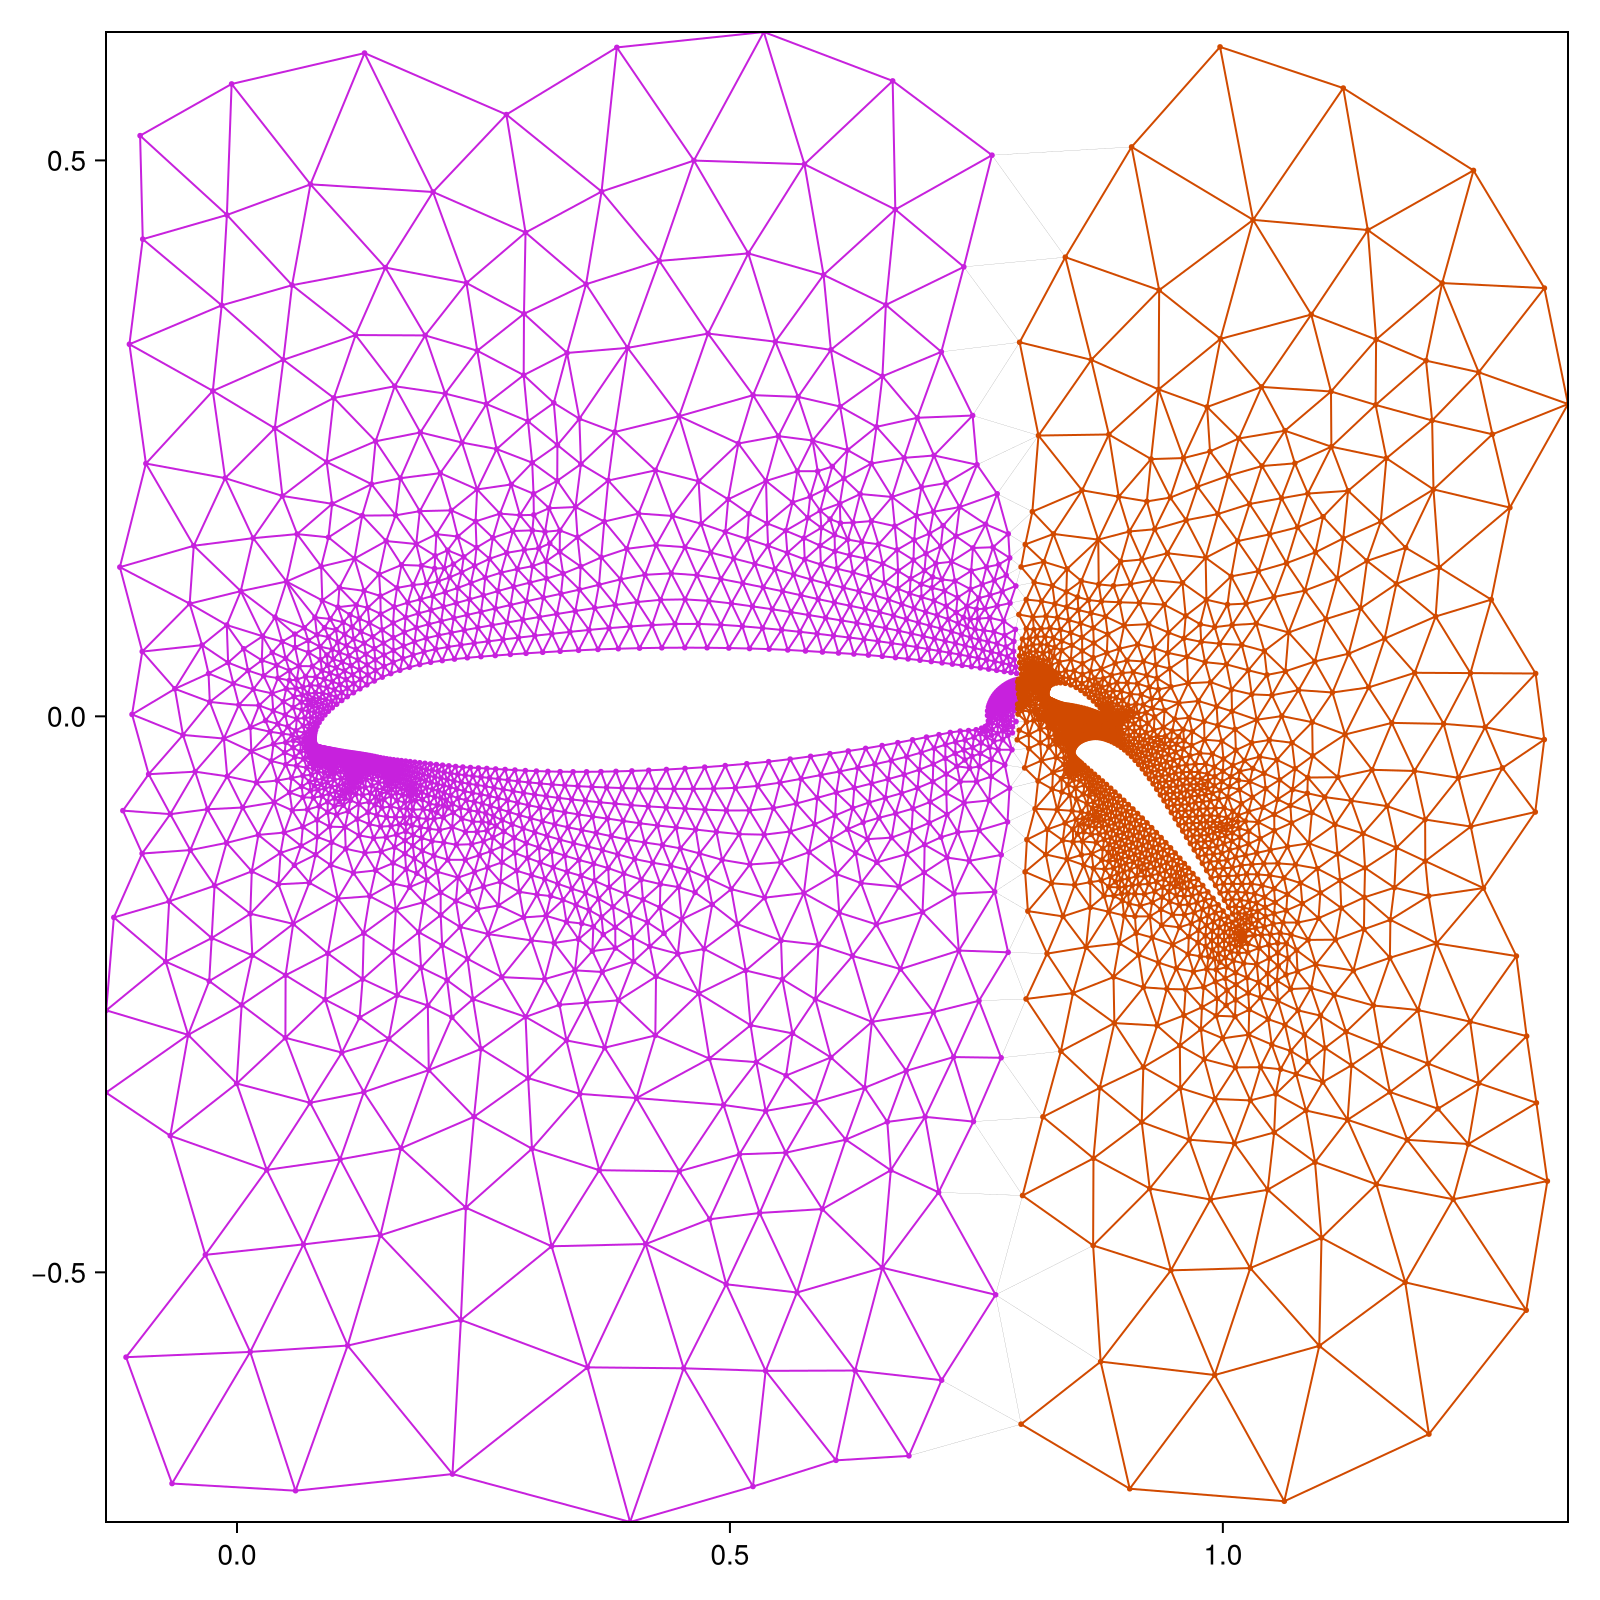
\includegraphics[width=\textwidth,  trim={100pt 74pt 0 0}, clip]{images/ex1_airfoil1_coordinate.png}
        \caption{Coordinate bisection}
        \label{fig:ex1_coord}
    \end{subfigure}
    \hfill
    \begin{subfigure}[b]{0.23\textwidth}
        \centering
        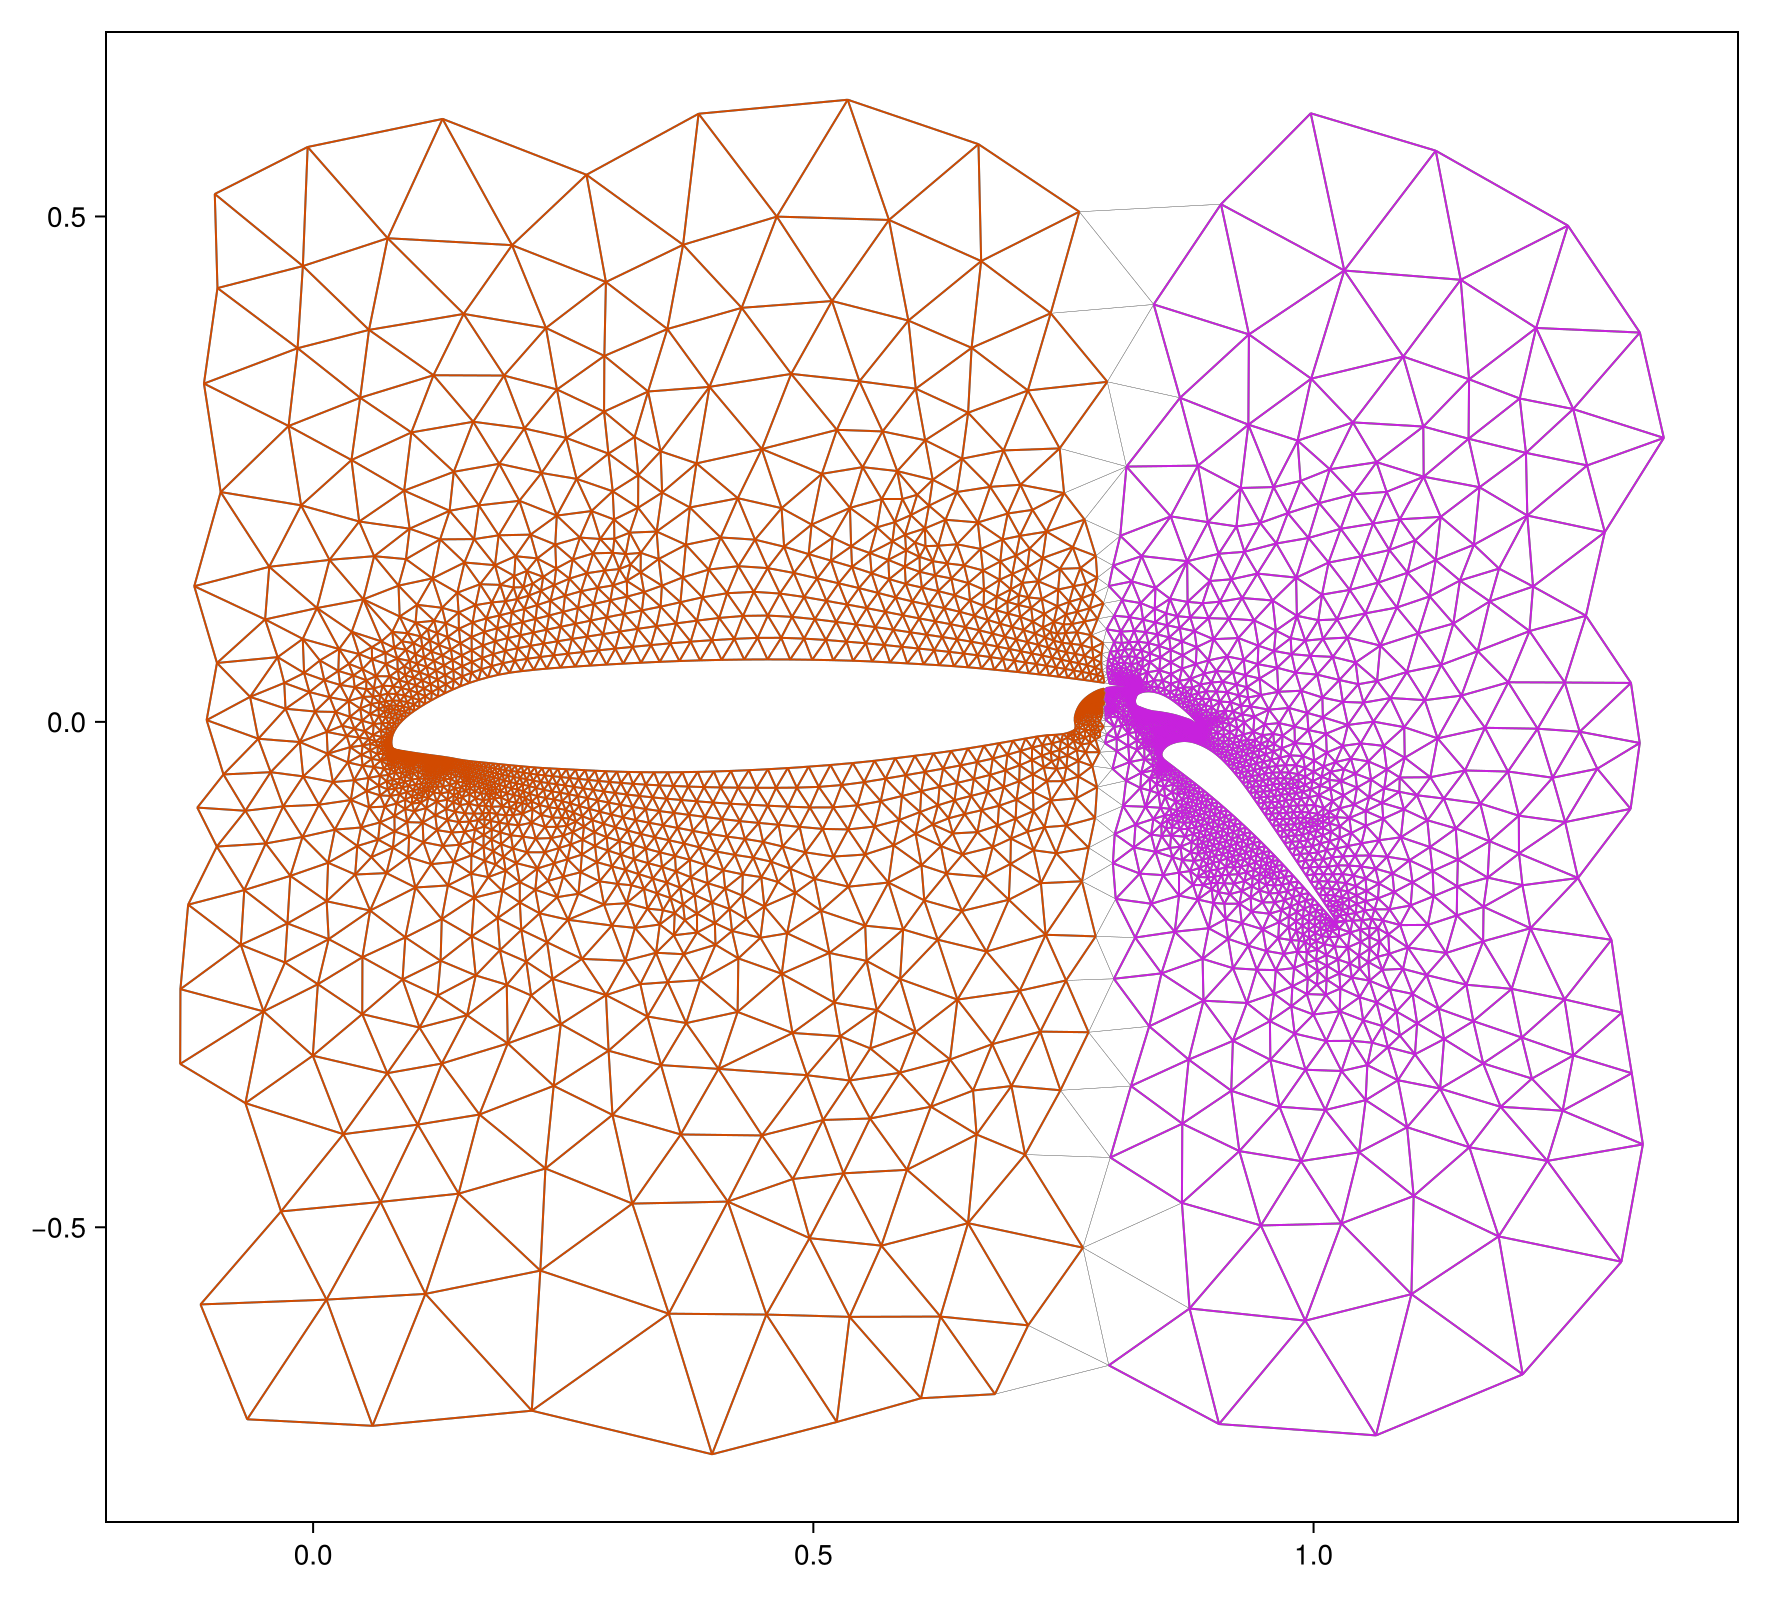
\includegraphics[width=\textwidth,  trim={100pt 74pt 0 0}, clip]{images/ex1_airfoil1_inertial.png}
        \caption{Inertial bisection}
        \label{fig:ex1_inertial}
    \end{subfigure}

    \vskip\baselineskip  % Adds vertical space between the rows

    \begin{subfigure}[b]{0.23\textwidth}
        \centering
        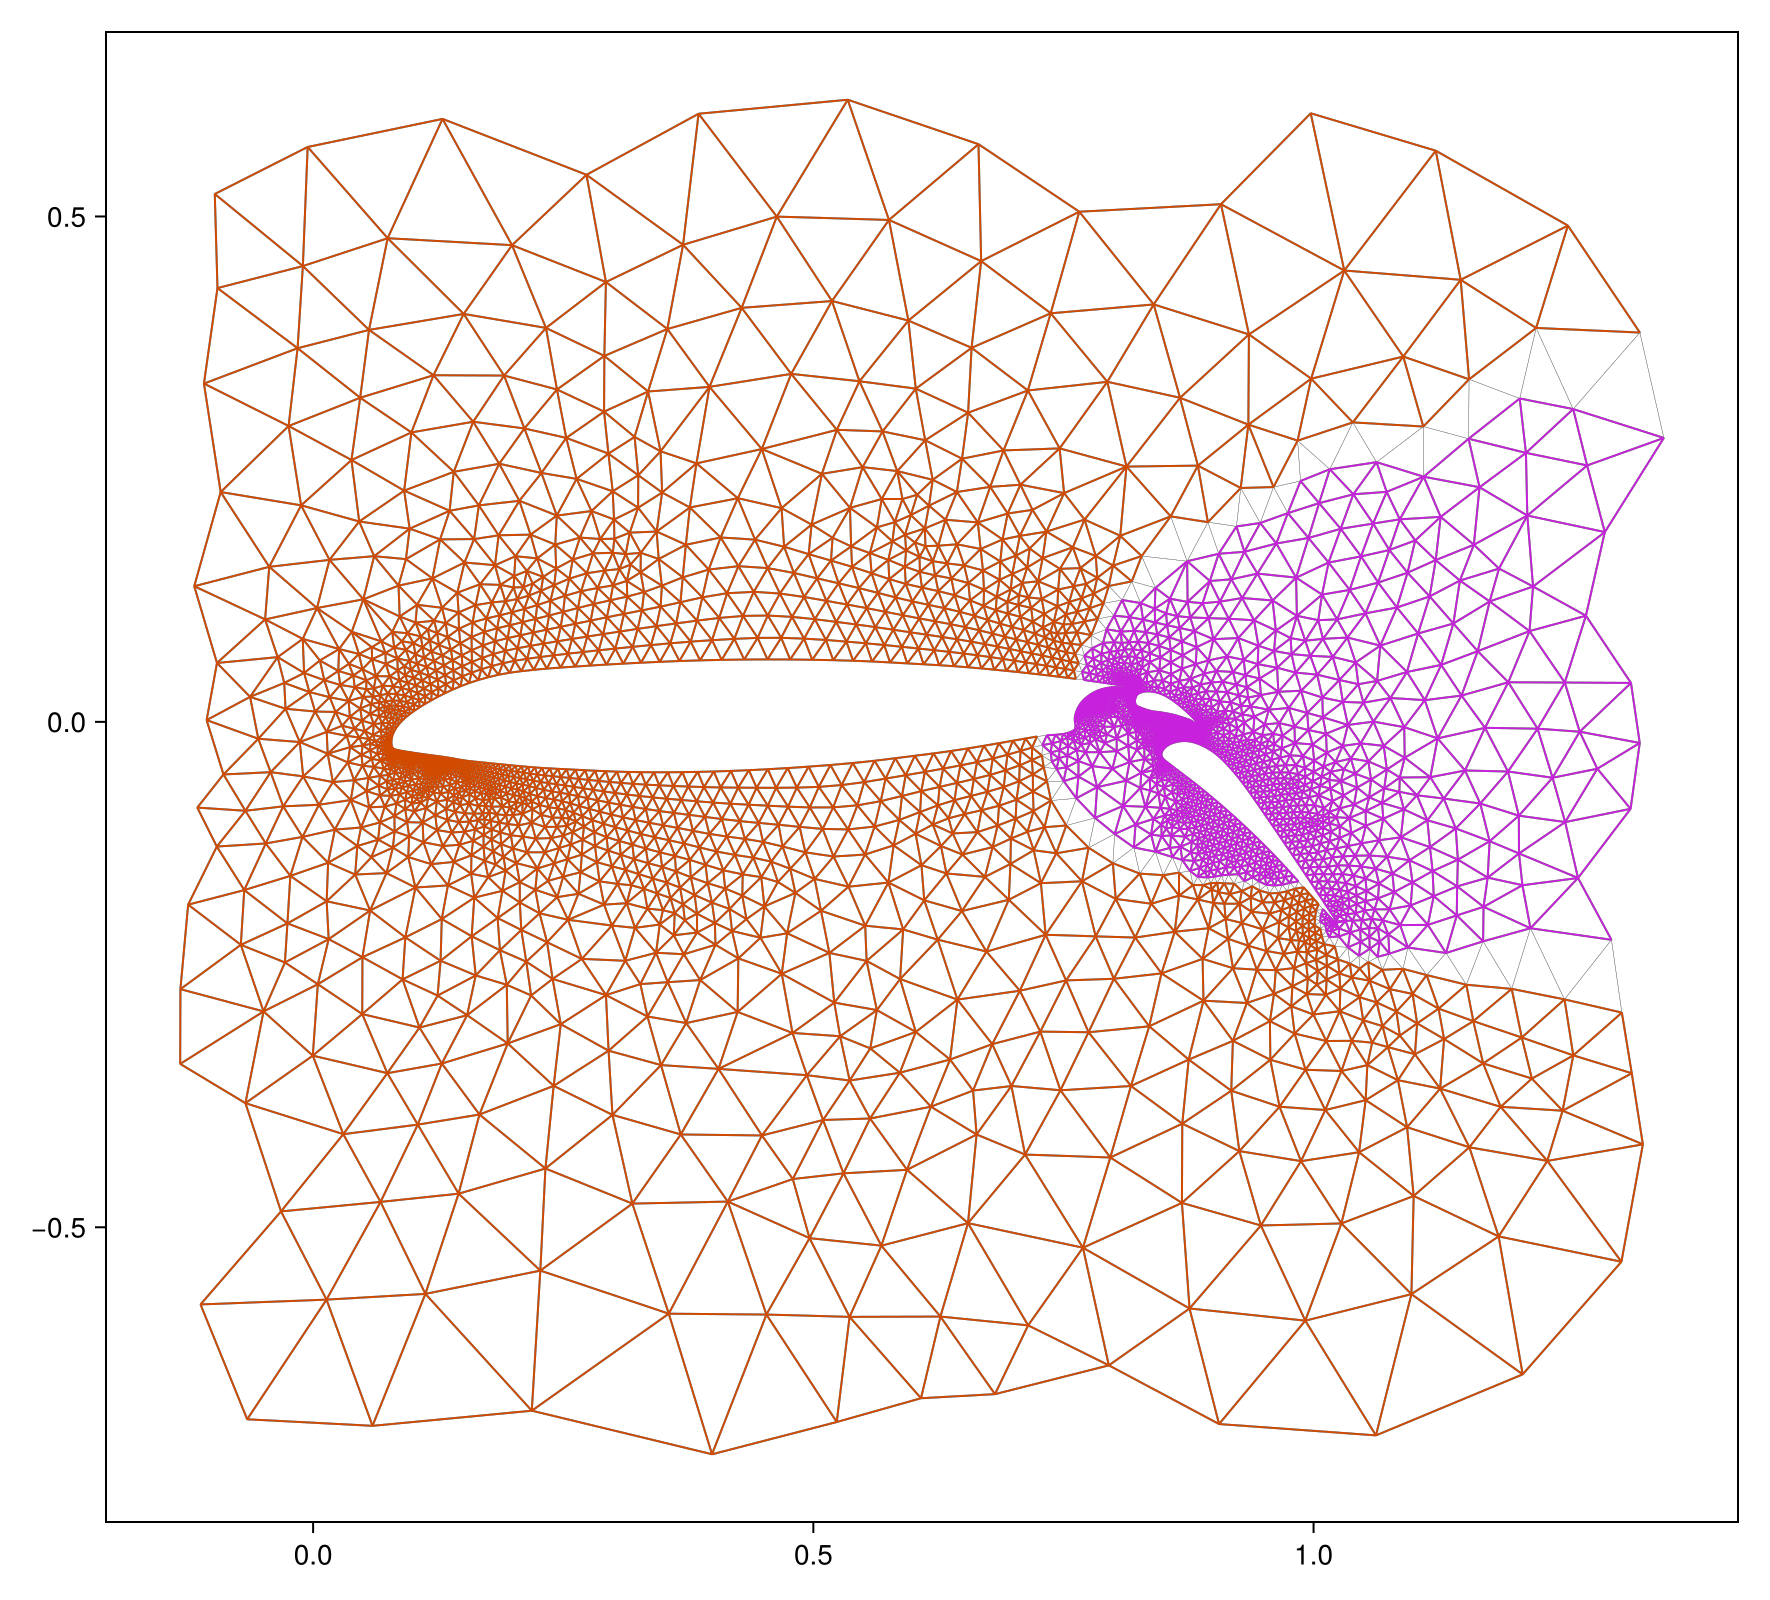
\includegraphics[width=\textwidth,  trim={100pt 74pt 0 0}, clip]{images/ex1_airfoil1_spectral.png}
        \caption{Spectral bisection}
        \label{fig:ex1_spectral}
    \end{subfigure}
    \hfill
    \begin{subfigure}[b]{0.23\textwidth}
        \centering
        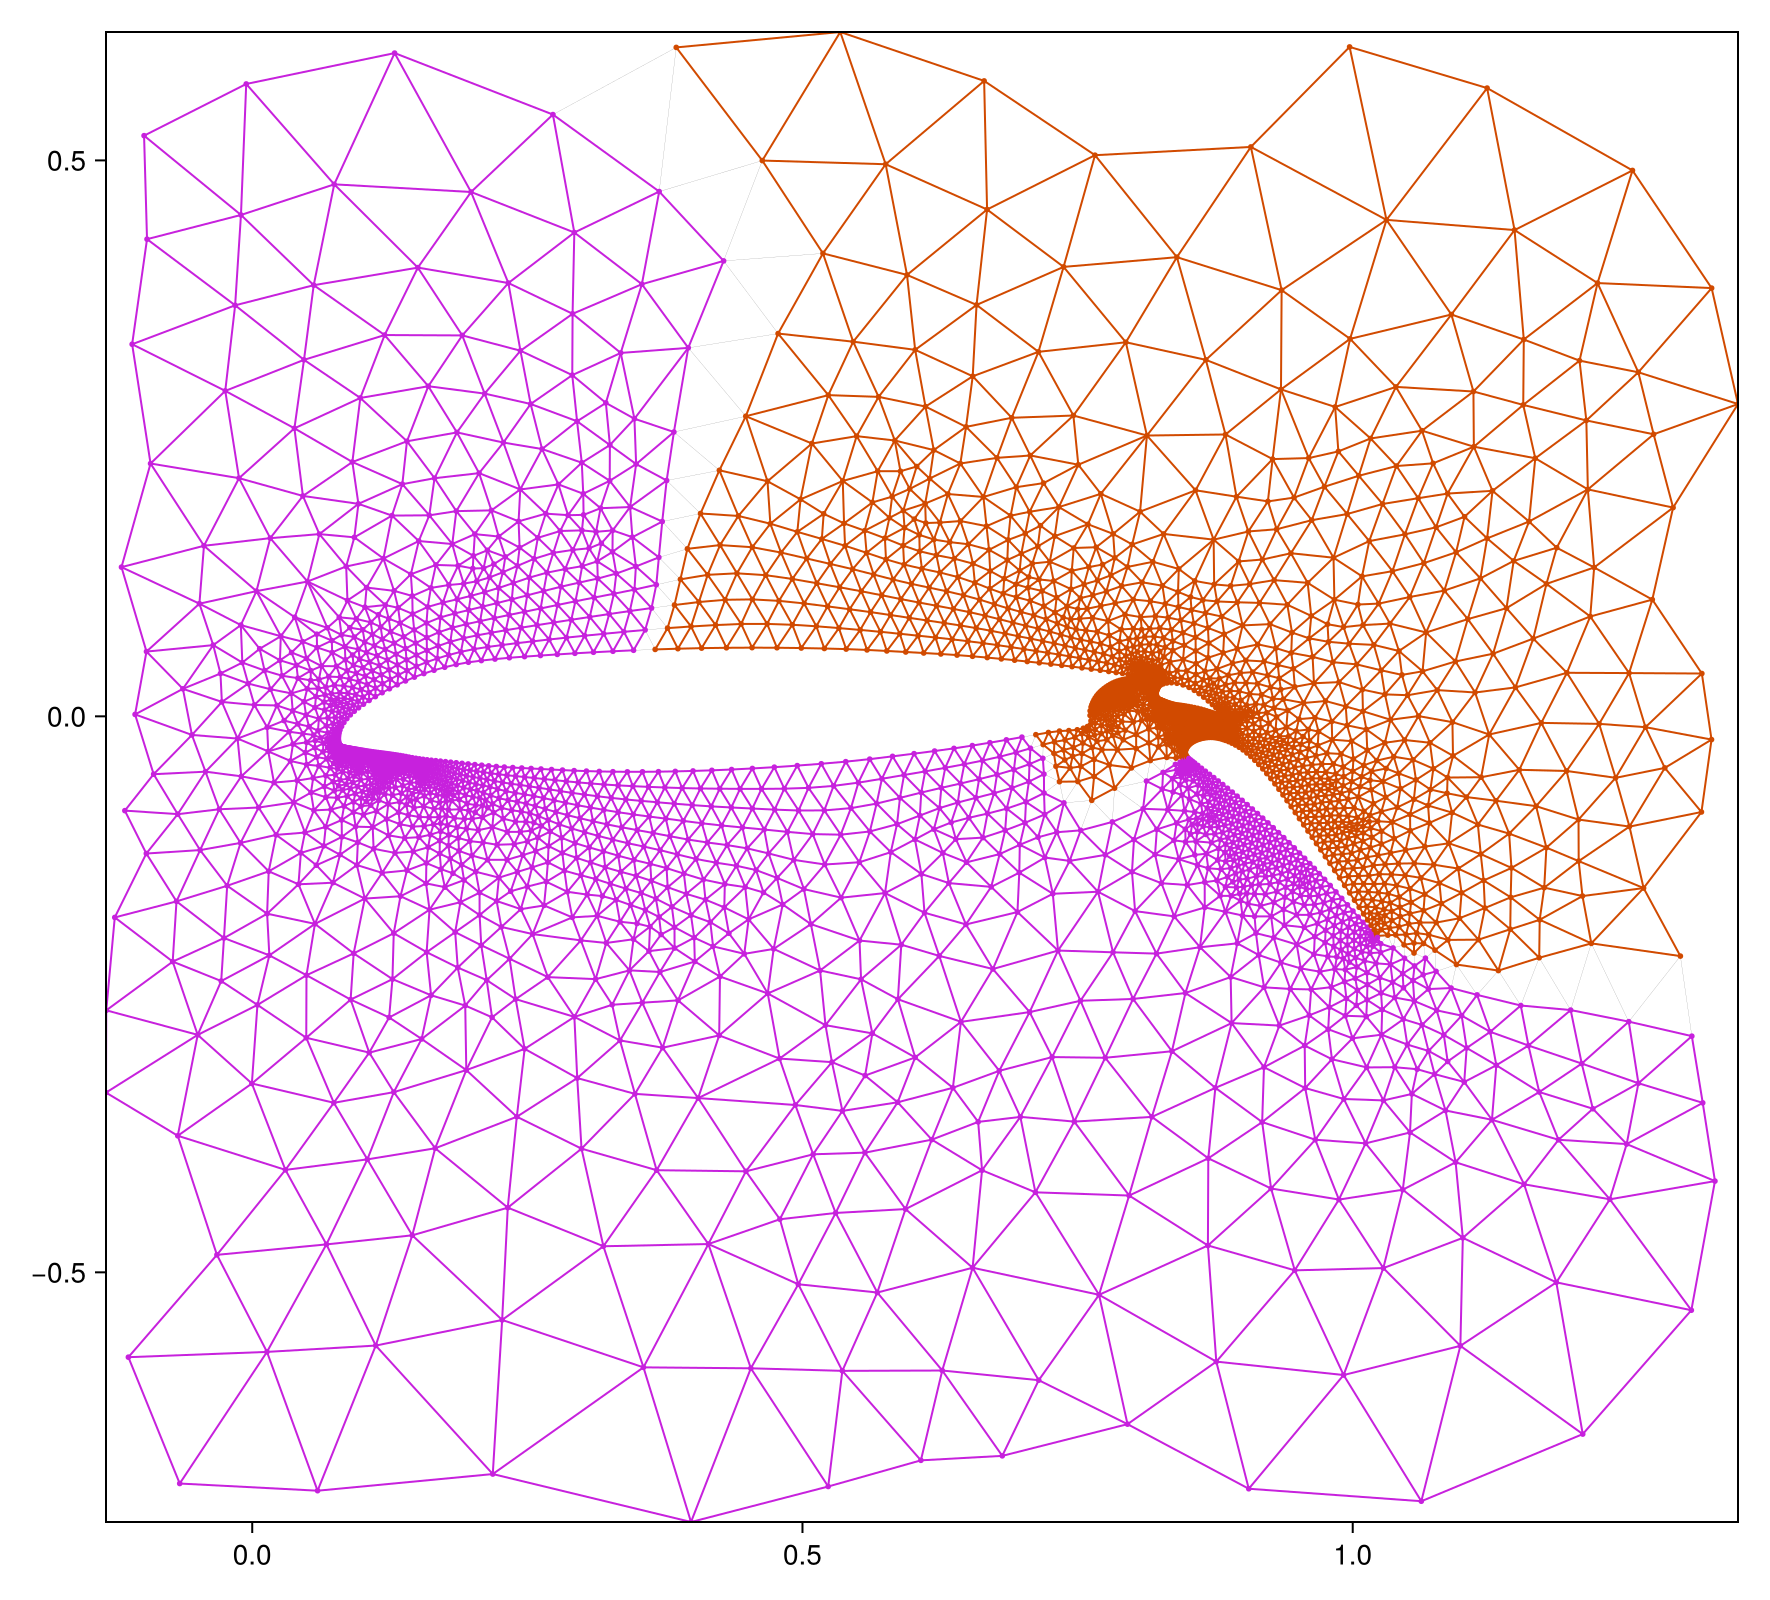
\includegraphics[width=\textwidth,  trim={100pt 74pt 0 0}, clip]{images/ex1_airfoil1_metis.png}
        \caption{Bisection using \texttt{METIS}}
        \label{fig:ex1_metis}
    \end{subfigure}

    \caption{Visualization of four graph bisection methods applied to the \texttt{airfoil1} mesh (4253 nodes and 12289 edges), illustrating differences in partitioning structure and edge cuts.}
    \label{fig:ex1_results}
\end{figure}


    \begin{figure}[h]
    \centering
    \begin{subfigure}[b]{0.23\textwidth}
        \centering
        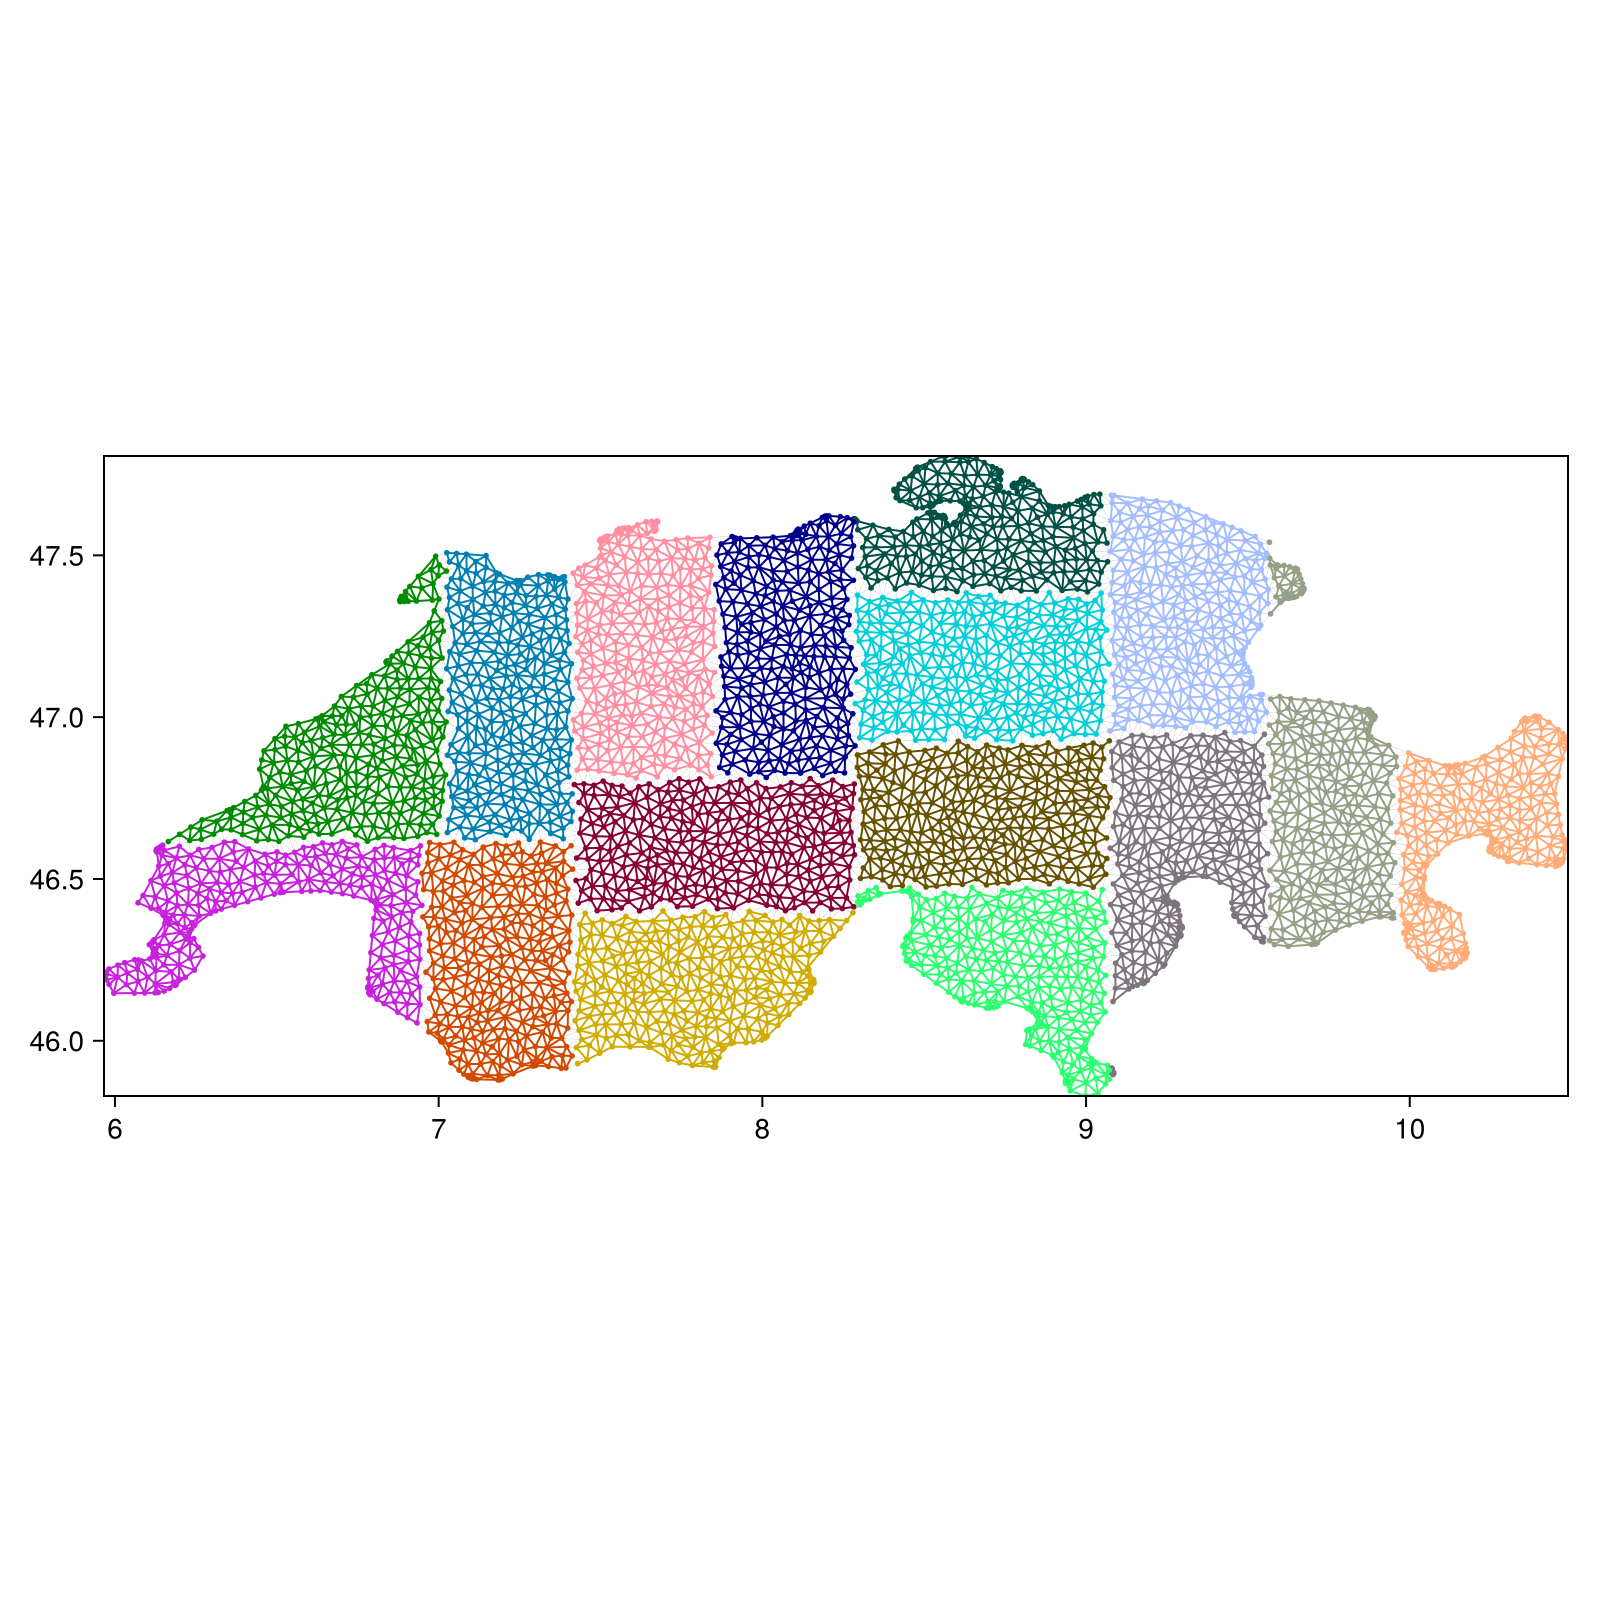
\includegraphics[width=\textwidth,  trim={98pt 70pt 0 0}, clip]{images/ex2_Swiss_graph_coordinate.png}
        \caption{Recursive coordinate bisection}
        \label{fig:ex2_coord}
    \end{subfigure}
    \hfill
    \begin{subfigure}[b]{0.23\textwidth}
        \centering
        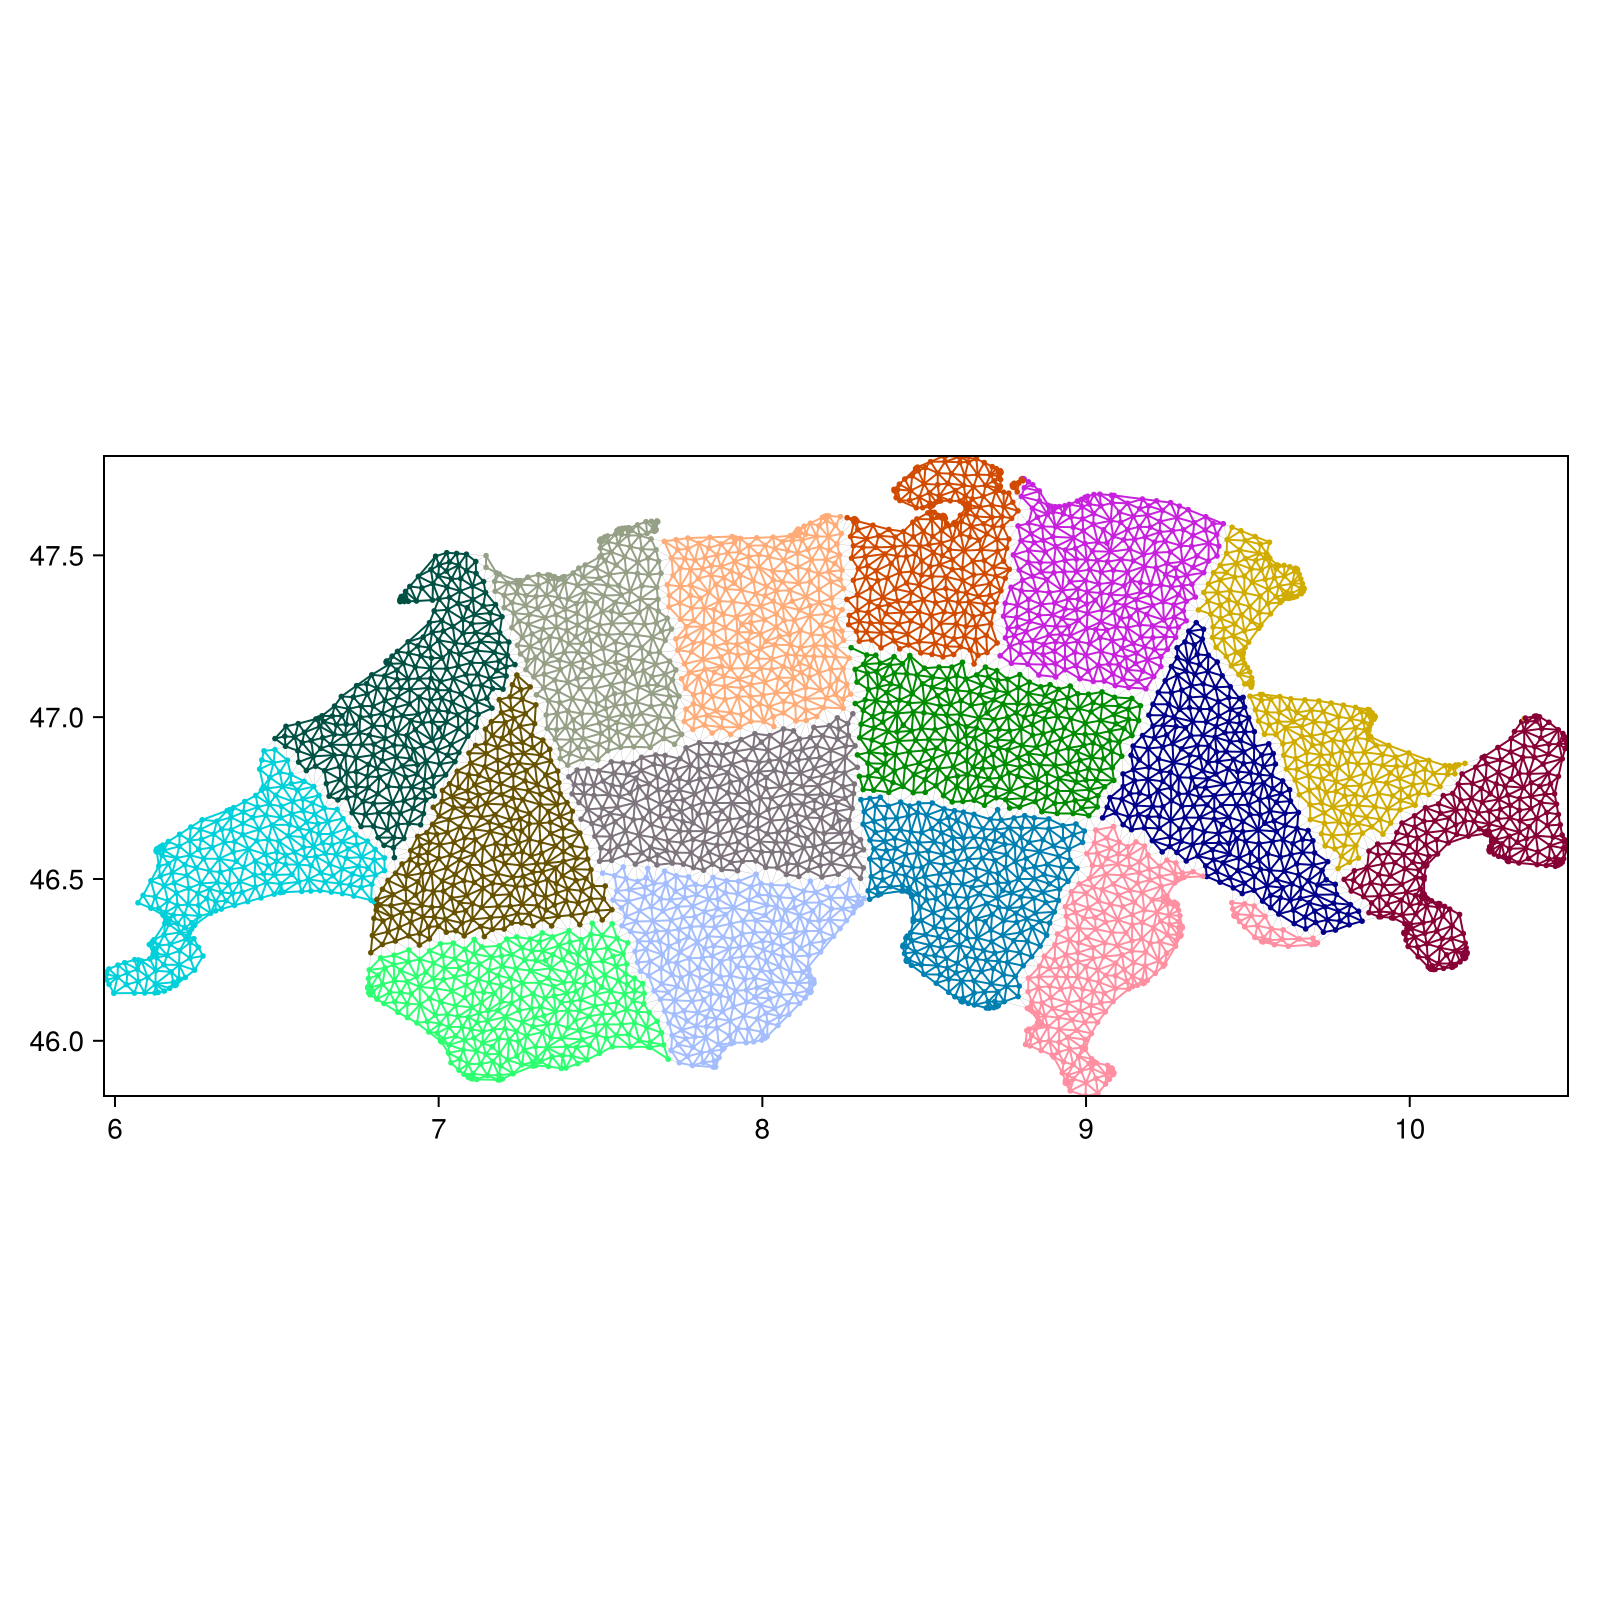
\includegraphics[width=\textwidth,  trim={98pt 70pt 0 0}, clip]{images/ex2_Swiss_graph_inertial.png}
        \caption{Recursive inertial bisection}
        \label{fig:ex2_inertial}
    \end{subfigure}

    \vskip\baselineskip  % Adds vertical space between the rows

    \begin{subfigure}[b]{0.23\textwidth}
        \centering
        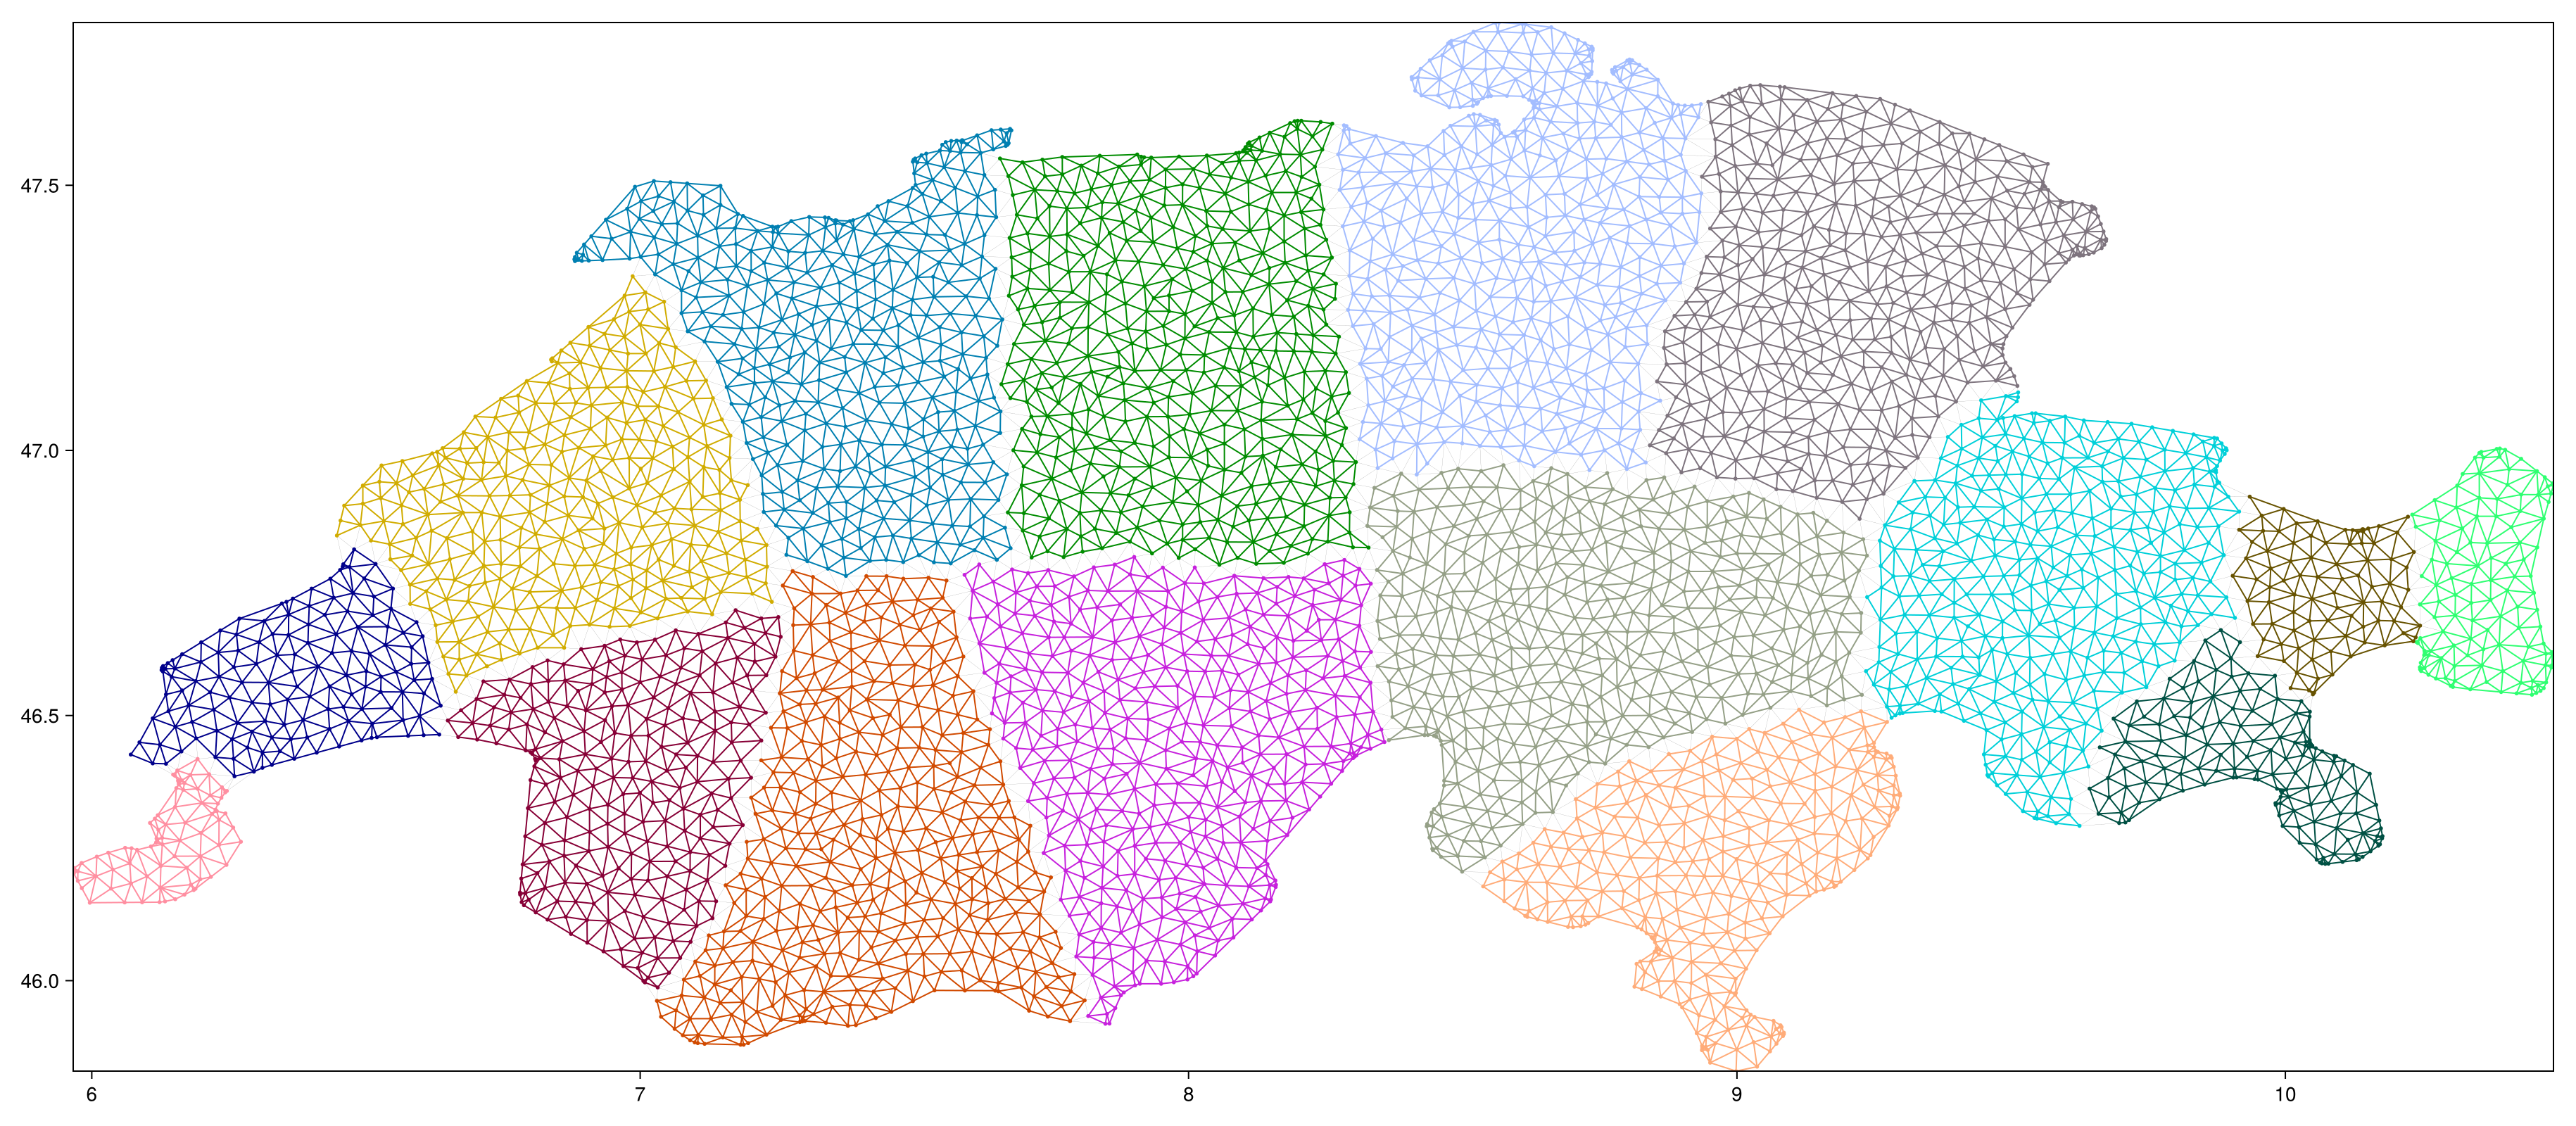
\includegraphics[width=\textwidth,  trim={98pt 70pt 0 0}, clip]{images/ex2_Swiss_graph_spectral.png}
        \caption{Recursive spectral bisection}
        \label{fig:ex2_spectral}
    \end{subfigure}
    \hfill
    \begin{subfigure}[b]{0.23\textwidth}
        \centering
        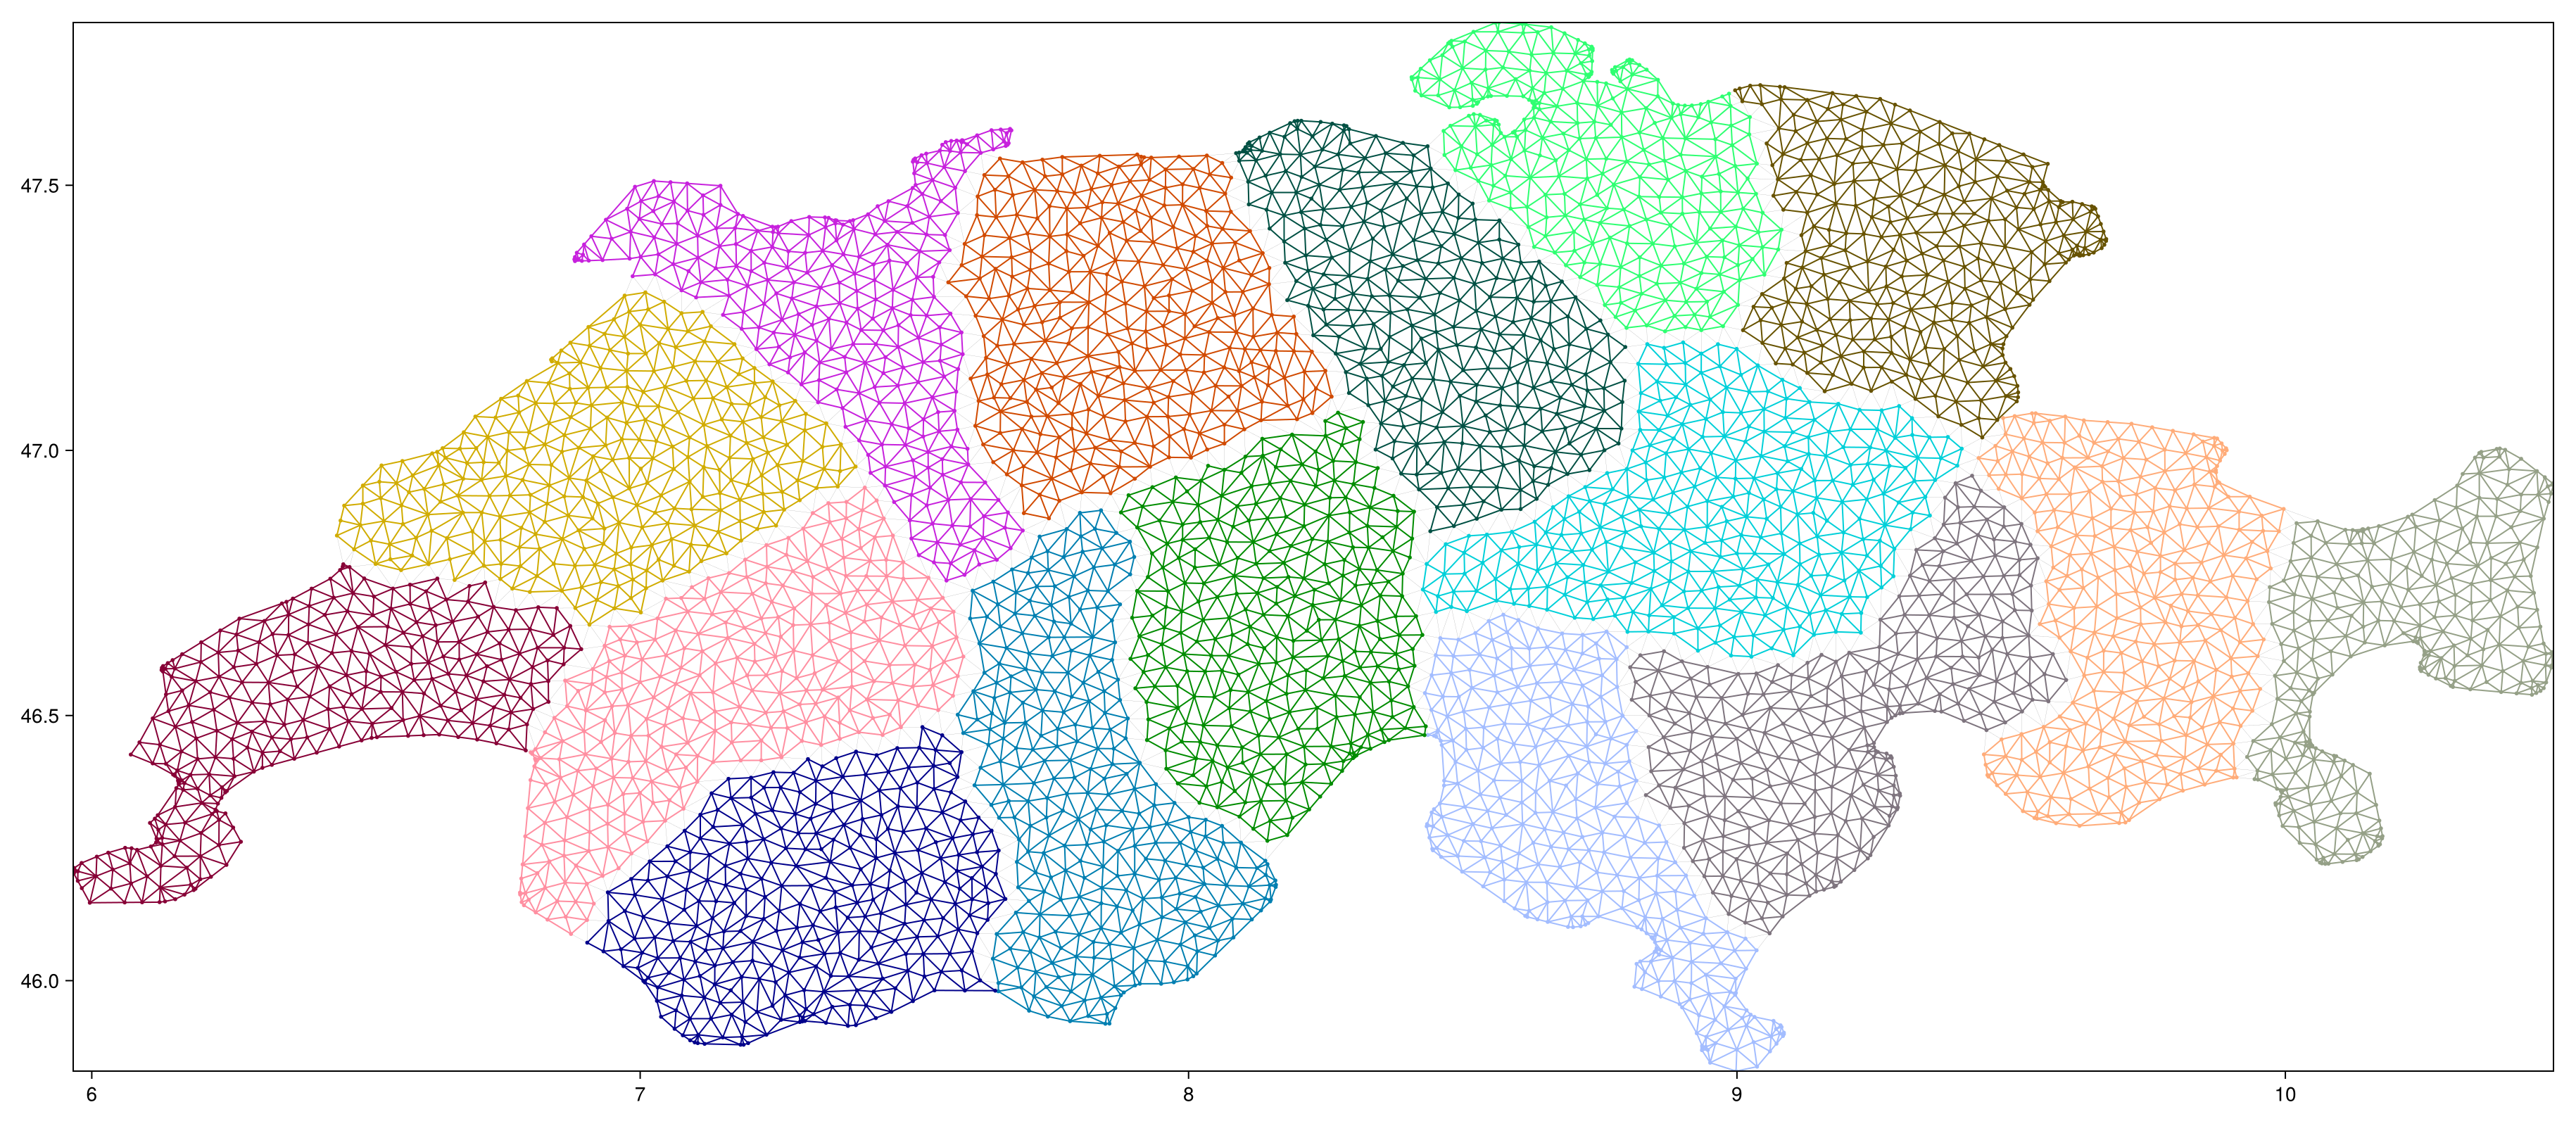
\includegraphics[width=\textwidth,  trim={98pt 70pt 0 0}, clip]{images/ex2_Swiss_graph_metis_rec.png}
        \caption{Recursive \texttt{METIS} bisection}
        \label{fig:ex2_metis}
    \end{subfigure}

    \caption{Comparison of four graph recursive bisection methods applied to the \texttt{Swiss\_graph} (4468 nodes and 15230 edges), illustrating differences in recursive partitioning results.}
    \label{fig:ex2_results}
\end{figure}


% \begin{figure}
%     \centering

%     \begin{subfigure}[b]{0.45\textwidth}
%         \centering
%         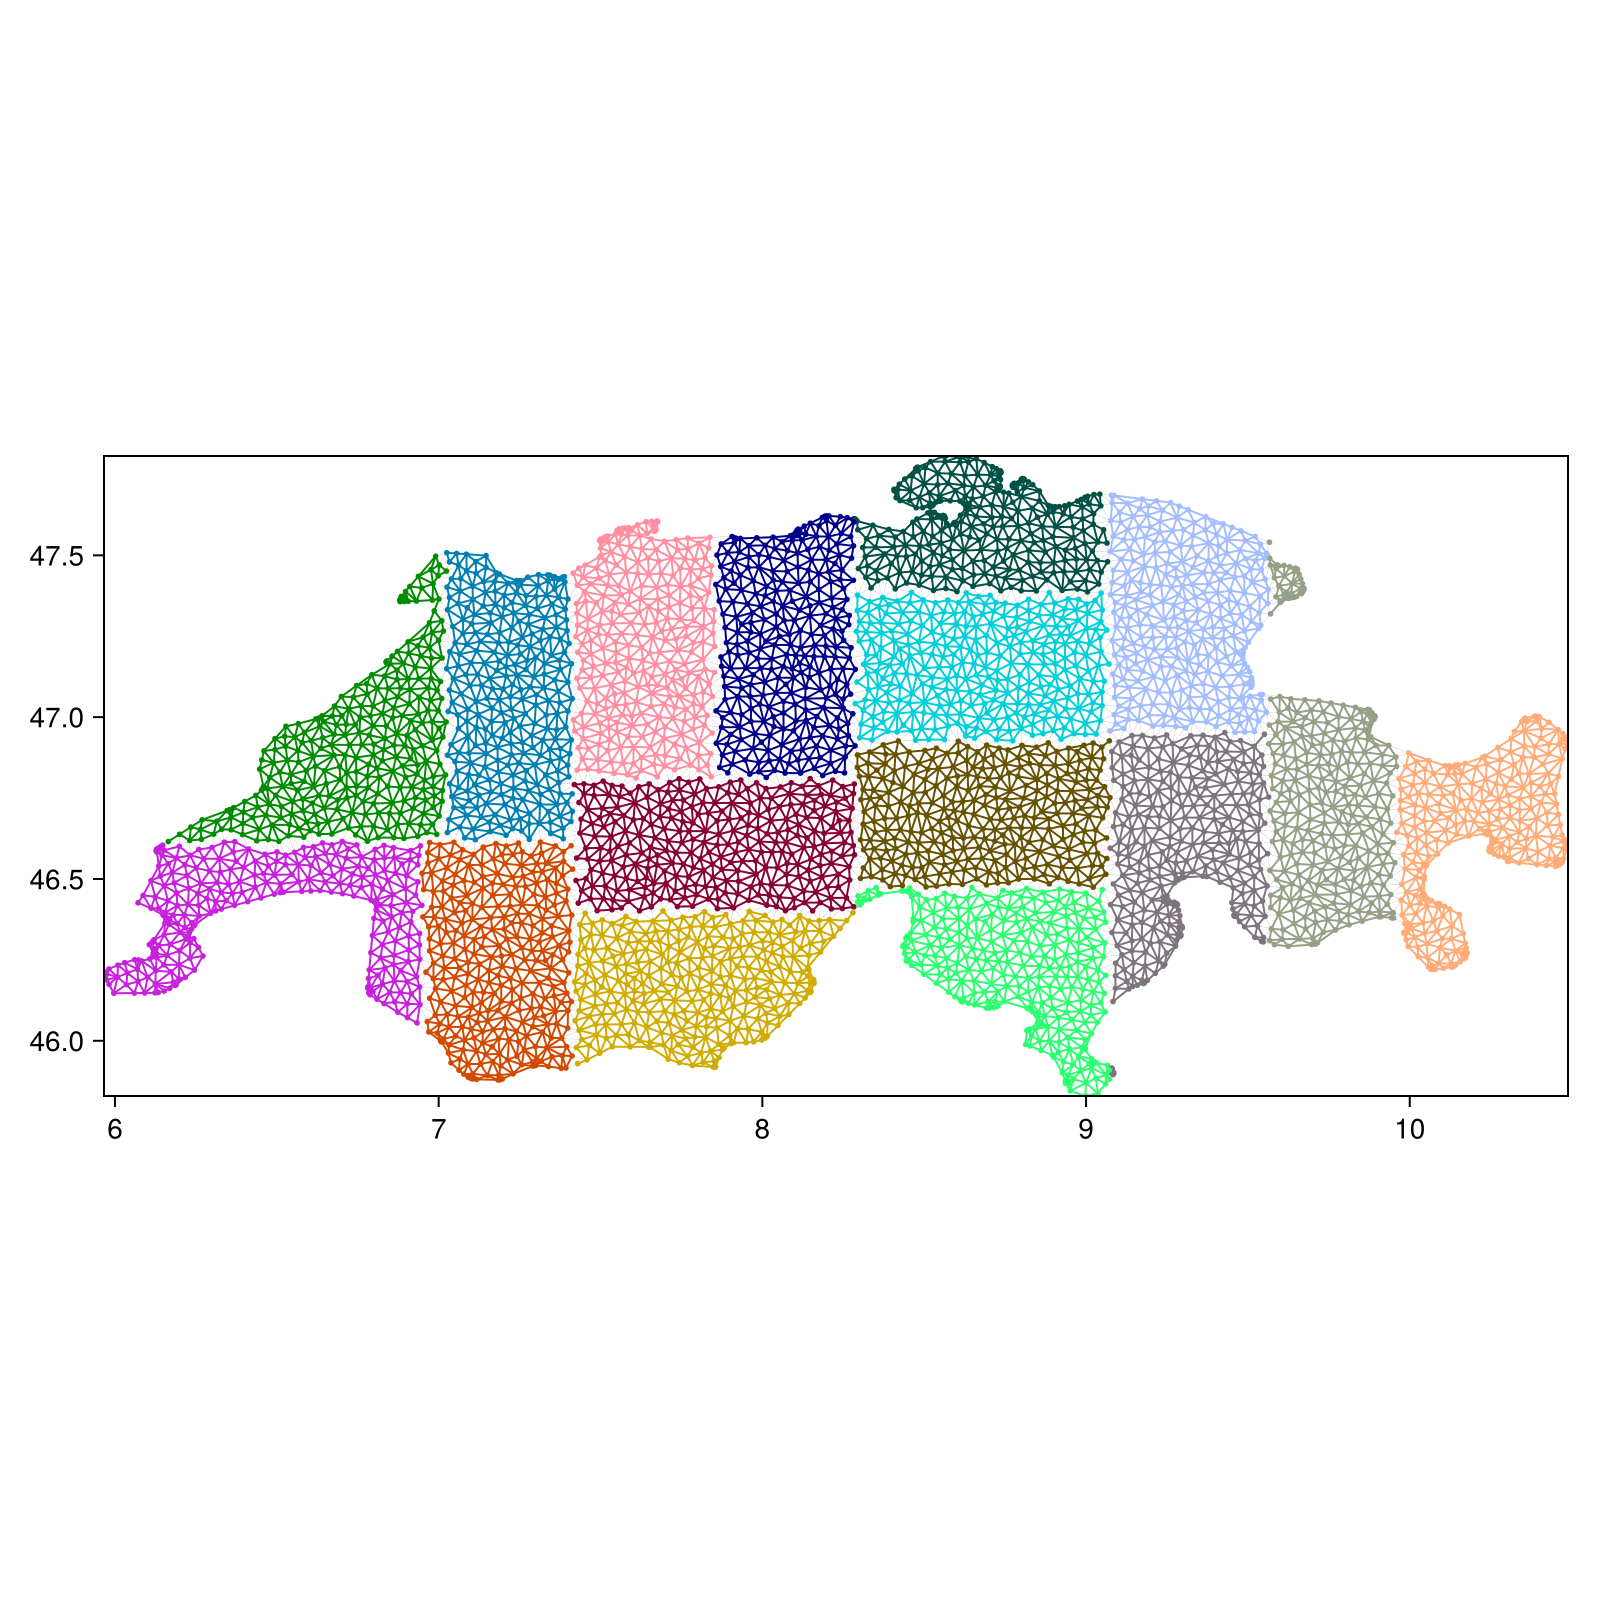
\includegraphics[width=\textwidth, trim={98pt 70pt 0 0}, clip]{images/ex2_Swiss_graph_coordinate.png}
%         \caption{Recursive coordinate bisection}
%         \label{fig:ex2_coord}
%     \end{subfigure}

%     \vskip\baselineskip

%     \begin{subfigure}[b]{0.45\textwidth}
%         \centering
%         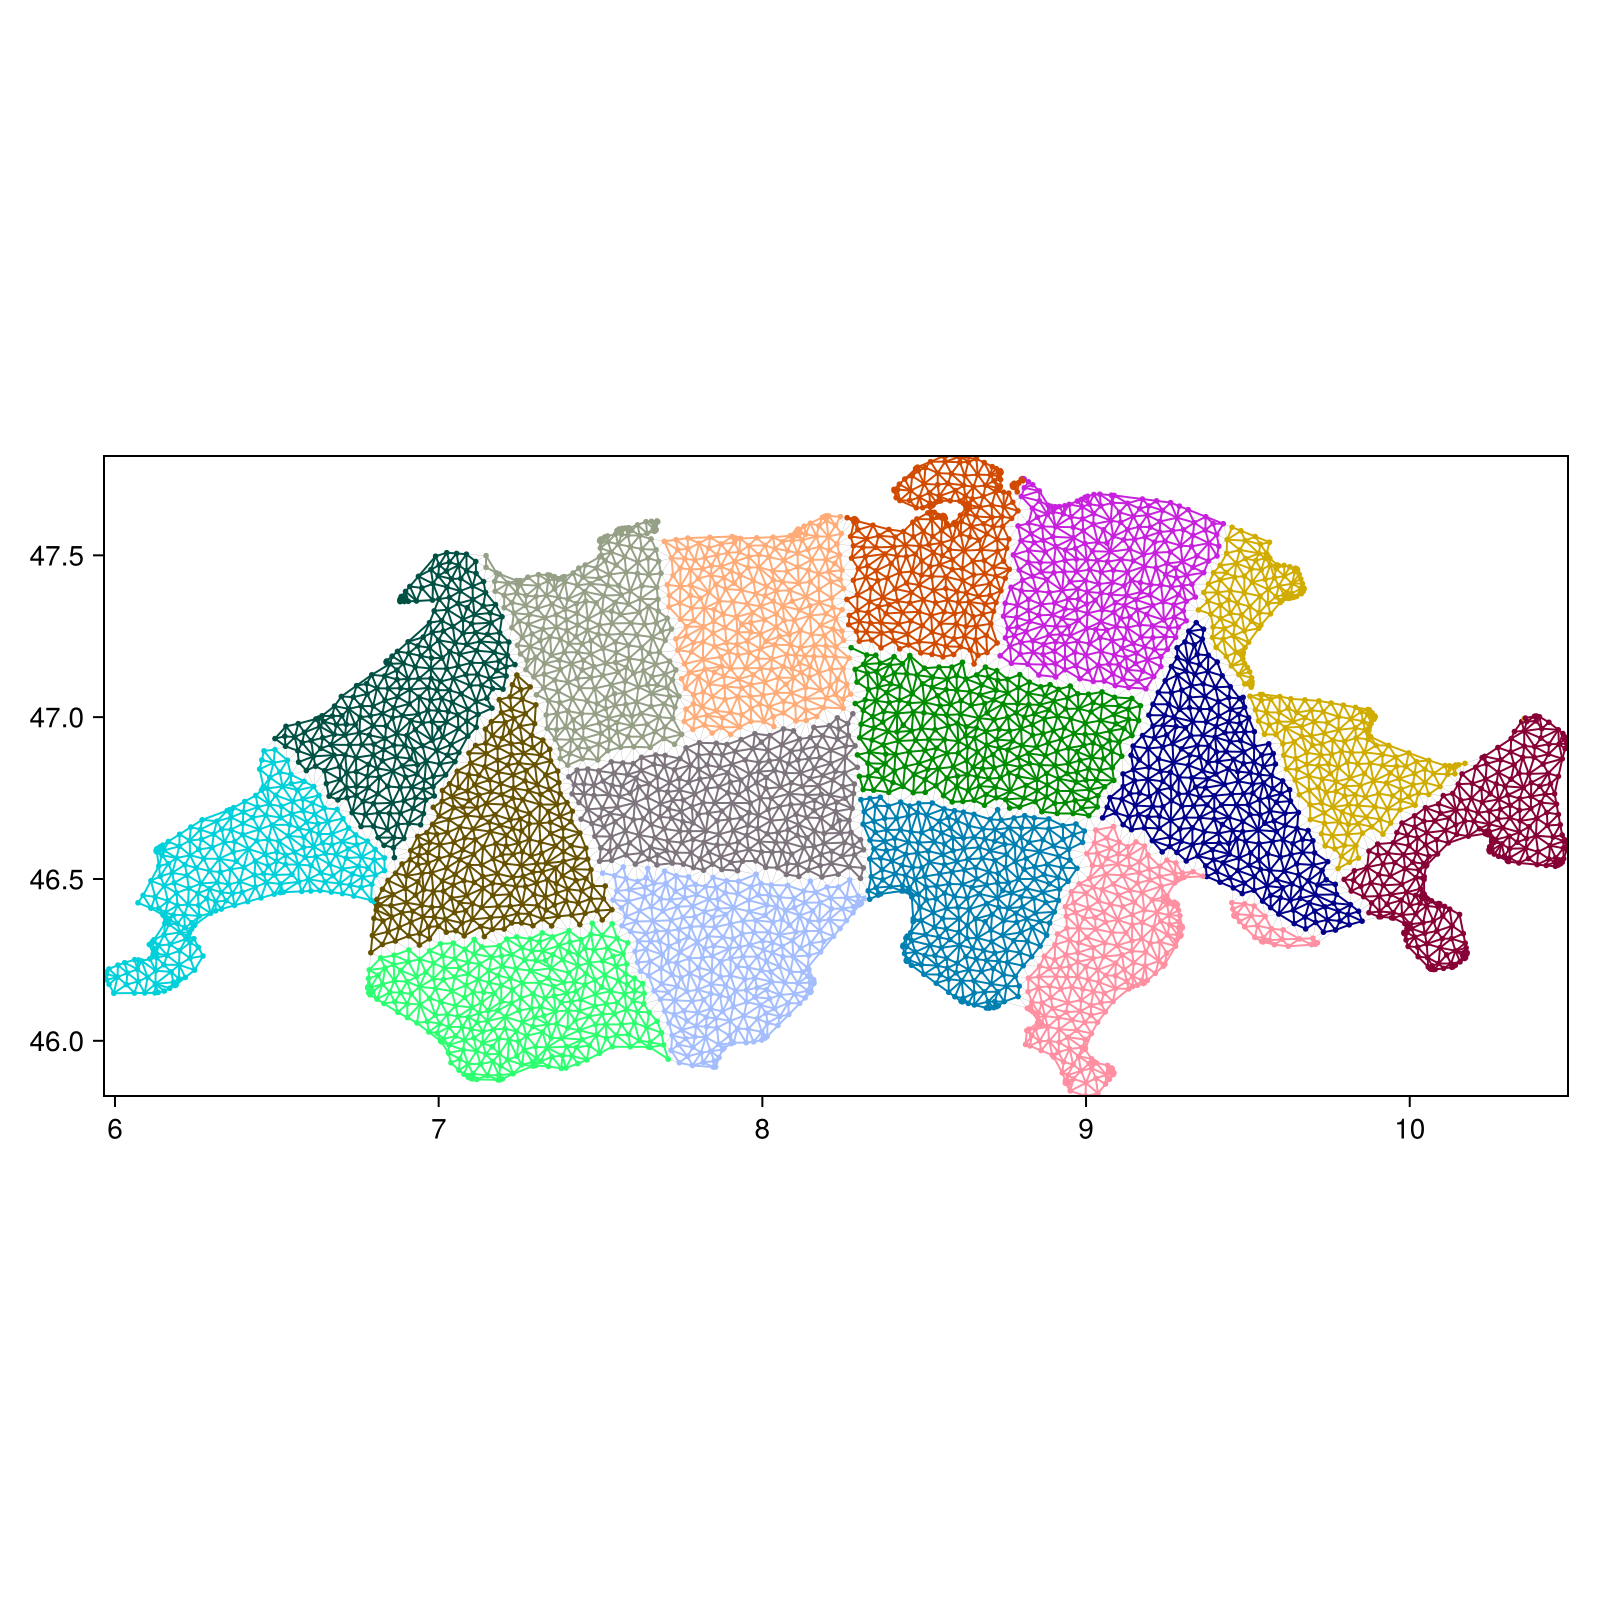
\includegraphics[width=\textwidth, trim={98pt 70pt 0 0}, clip]{images/ex2_Swiss_graph_inertial.png}
%         \caption{Recursive inertial bisection}
%         \label{fig:ex2_inertial}
%     \end{subfigure}

%     \vskip\baselineskip

%     \begin{subfigure}[b]{0.45\textwidth}
%         \centering
%         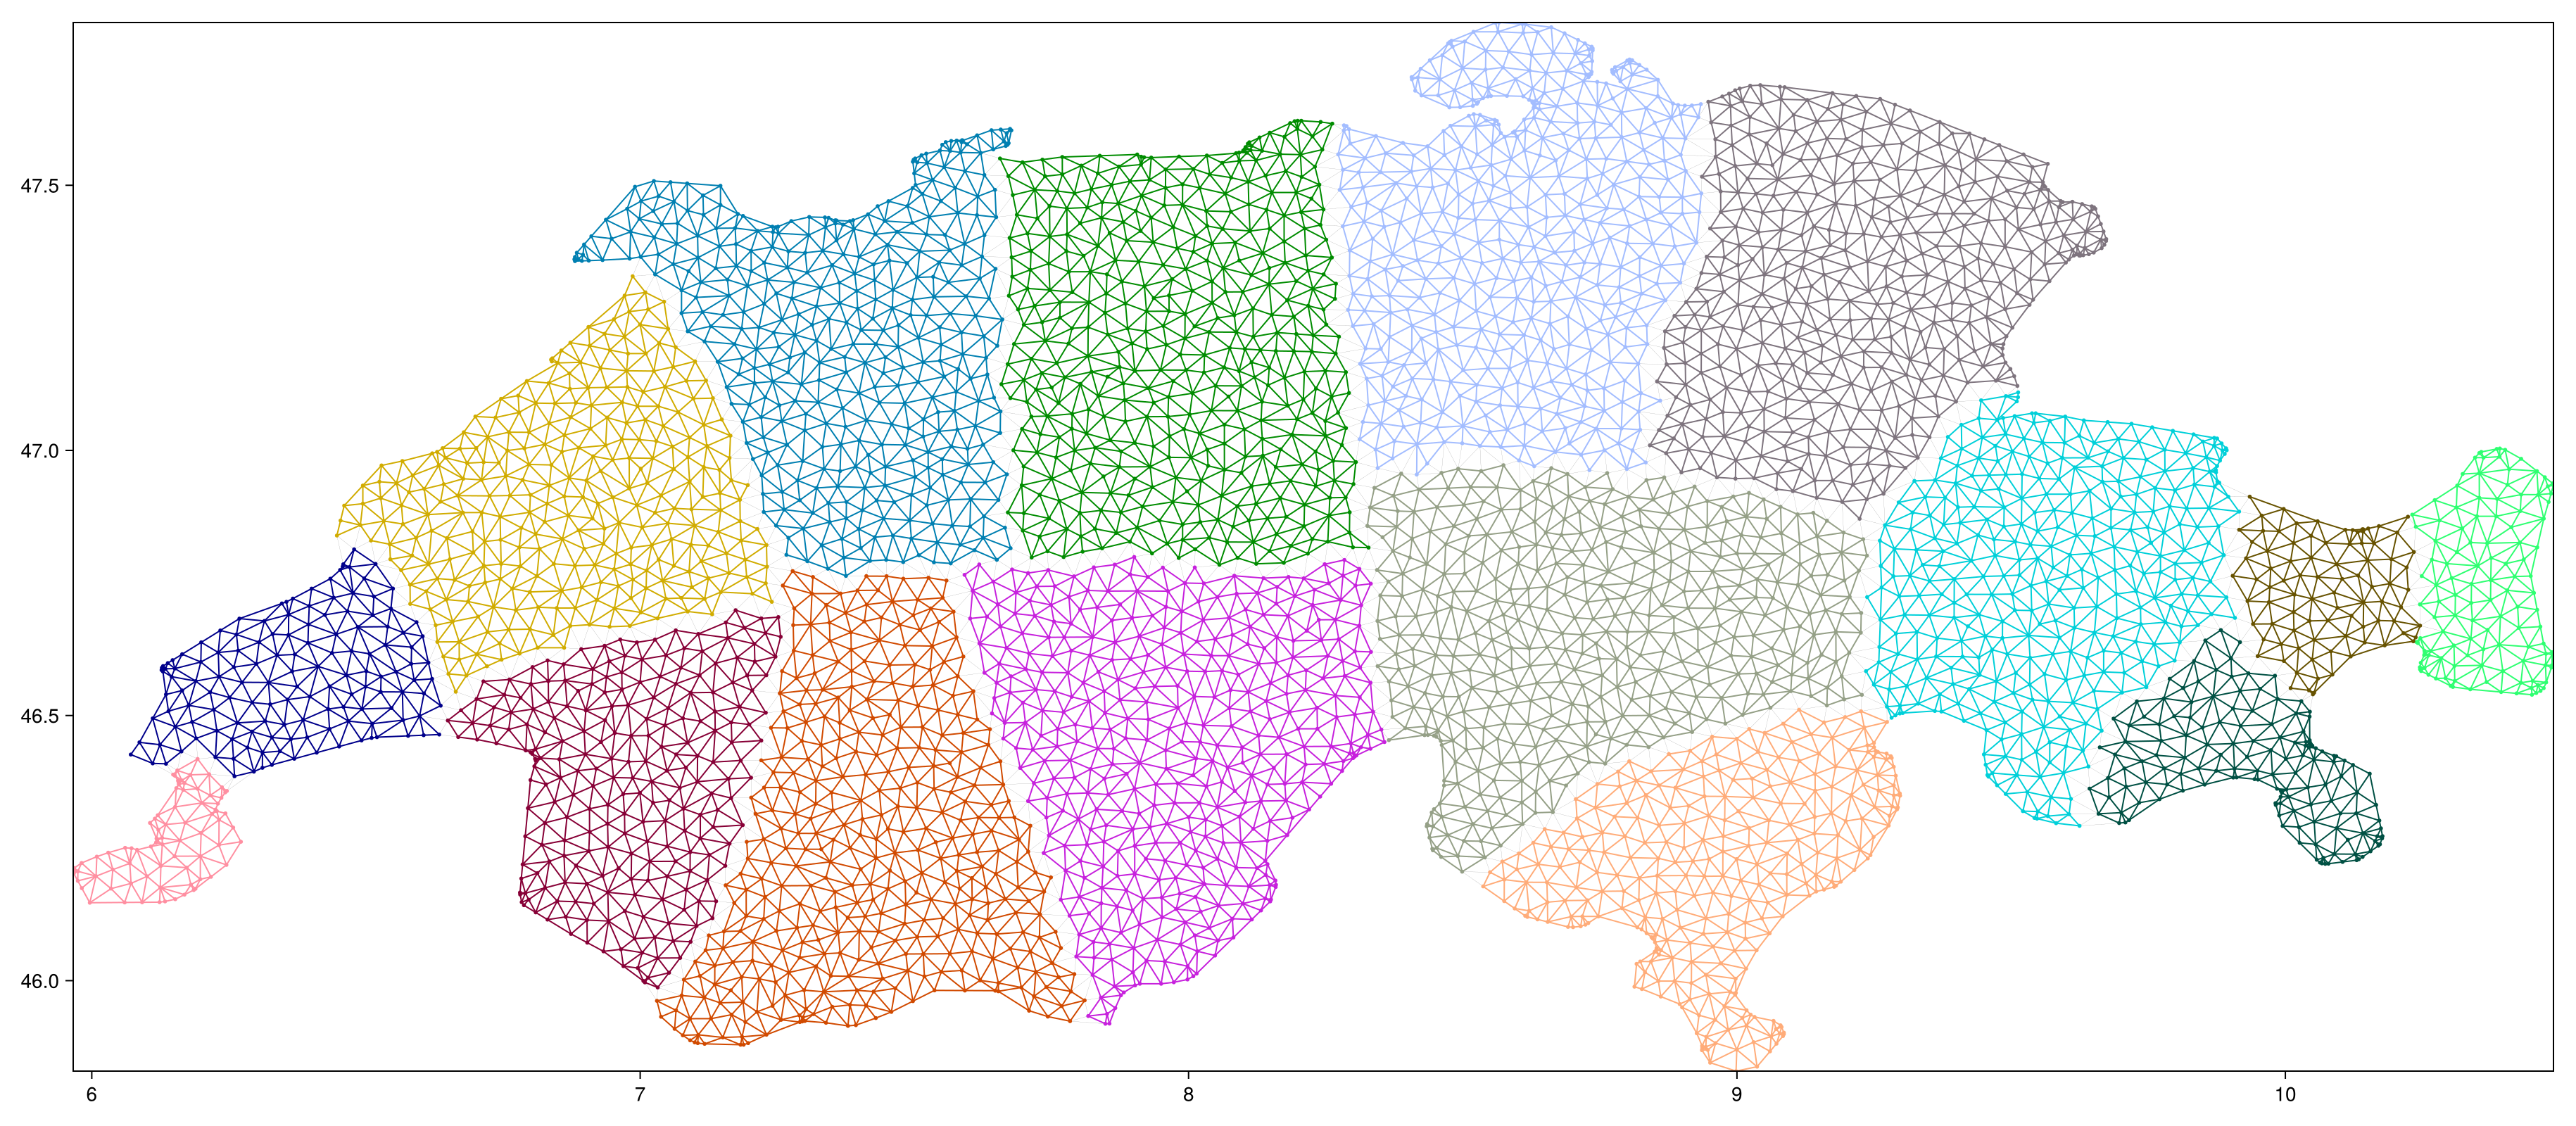
\includegraphics[width=\textwidth, trim={98pt 70pt 0 0}, clip]{images/ex2_Swiss_graph_spectral.png}
%         \caption{Recursive spectral bisection}
%         \label{fig:ex2_spectral}
%     \end{subfigure}

%     \vskip\baselineskip

%     \begin{subfigure}[b]{0.45\textwidth}
%         \centering
%         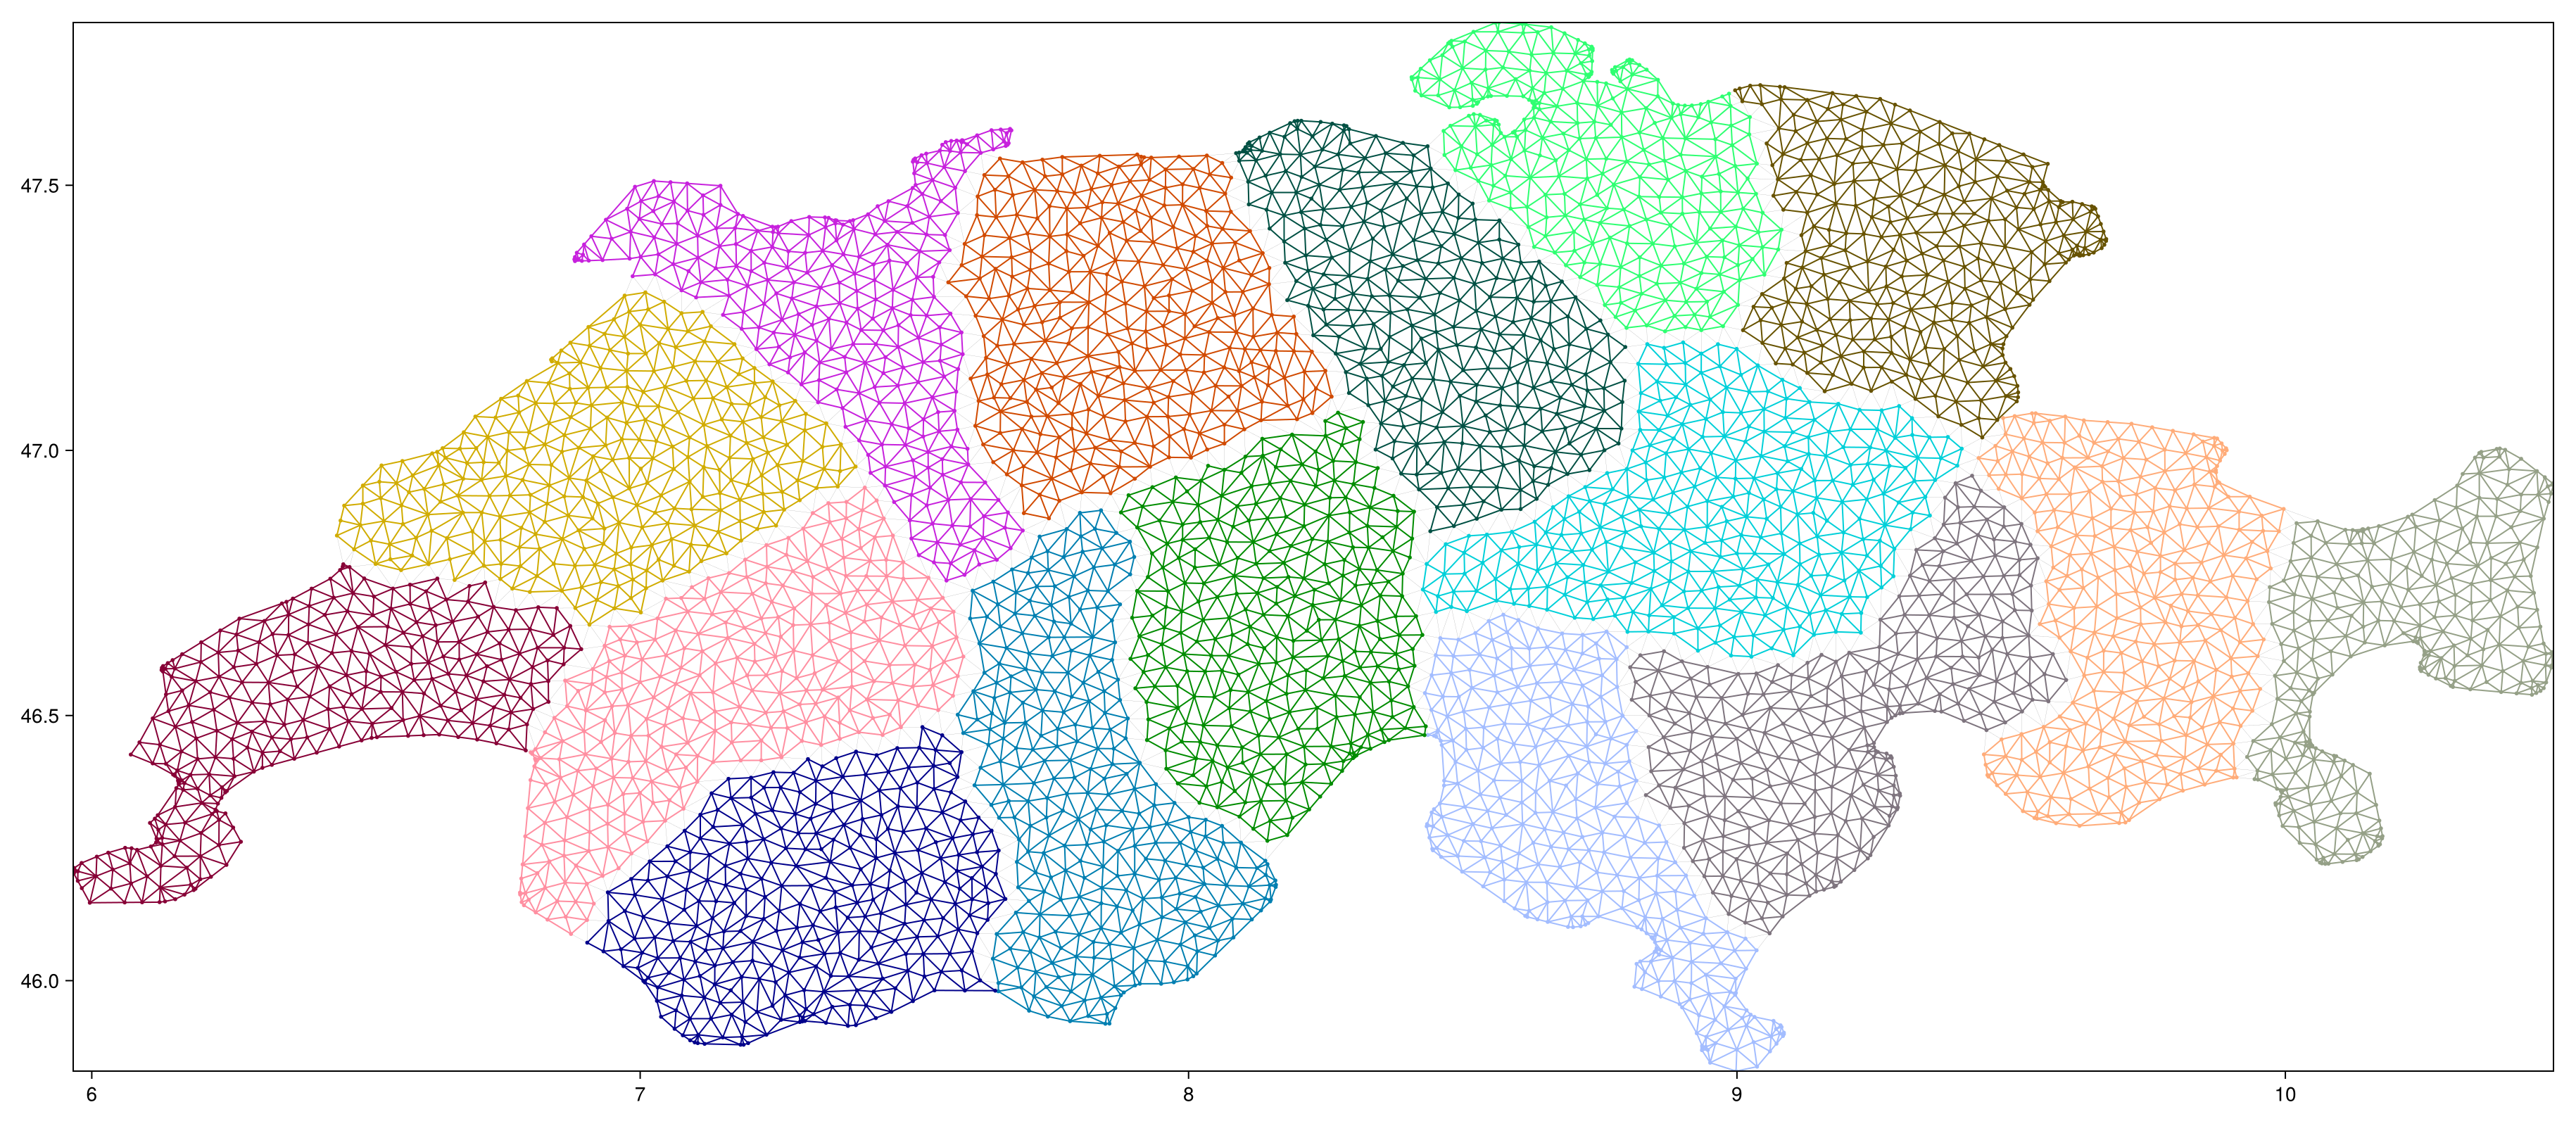
\includegraphics[width=\textwidth, trim={98pt 70pt 0 0}, clip]{images/ex2_Swiss_graph_metis_rec.png}
%         \caption{Recursive spectral bisection}
%         \label{fig:ex2_metis}
%     \end{subfigure}

%     \caption{Recursive bisection of the \texttt{Swiss\_graph} mesh using different methods. Each partition result shows the division into $p = 16$ subdomains.}
%     \label{fig:ex2_results}
% \end{figure}
   %  \begin{figure}[h!]
    \centering
    \begin{subfigure}[b]{0.23\textwidth}
        \centering
        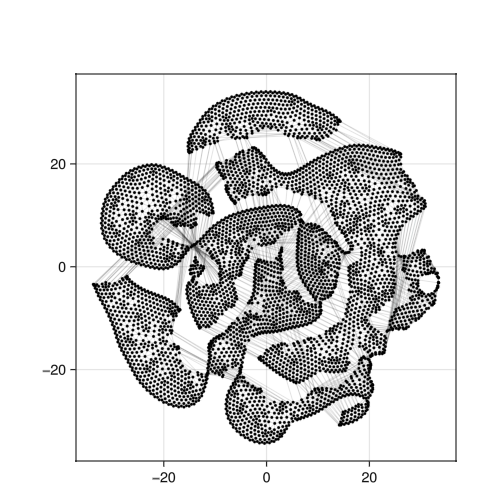
\includegraphics[trim={0 0 0 2.5cm}, clip, width=1.1\textwidth]{images/plot_ex_1.png}
        % \caption{}
        \label{fig:visu_simple}
    \end{subfigure}
    \hfill
    \begin{subfigure}[b]{0.23\textwidth}
        \centering
        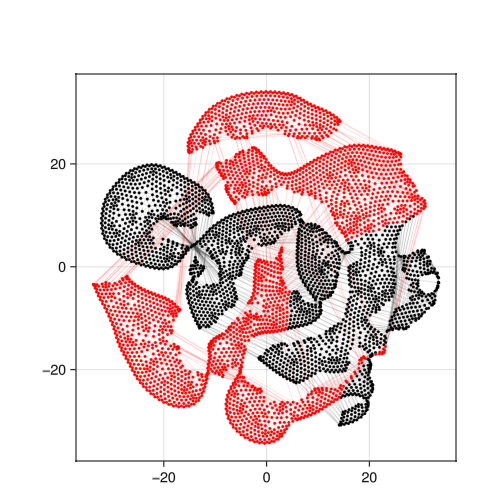
\includegraphics[trim={0 0 0 2.5cm}, clip, width=1.1\textwidth]{images/plot_ex_2.png}
        % \caption{}
        \label{fig:visu_2part}
    \end{subfigure}
    \caption{Graph visualization example and the corresponding result after applying
    a bisection. The original graph structure is shown on the left, while the right 
    visualization highlights the two obtained partitions.}
    \label{fig:visu}
\end{figure}
%%%%%%%%%%%%%%%%%%%%%%%%%%%%%%%%%%%%%%%%%%%%%%%%%%%%%%%%%%%%%%
% Integration
%%%%%%%%%%%%%%%%%%%%%%%%%%%%%%%%%%%%%%%%%%%%%%%%%%%%%%%%%%%%%%
    % \subsection{Integration with external graph partitioning software}
    % \label{subsec:integr}
    % The framework supports interoperability with widely used graph partitioning tools, allowing
    % users to incorporate advanced algorithms alongside the provided methods.
    % We provide guidelines and examples demonstrating how to integrate external software into
    % \texttt{GraphLab.jl}.
    % The proposed integration workflow follows these steps:

    %     \begin{enumerate}
    %         \item \textbf{Graph file generation}: Convert the symmetric adjacency matrix into a format compatible with external tools. The standard format includes:
    %             \begin{itemize}
    %                 \item The first line specifying the number of nodes and edges.
    %                 \item Each subsequent line representing a node, listing its neighbors as space-separated integers.
    %             \end{itemize}
                
    %         \item \textbf{Executable path retrieval and validation}: Retrieve the path of the external partitioning software from environment variables and ensure its existence.
            
    %         \item \textbf{Error handling}: Verify the exit code to detect execution failures or misconfigurations.
            
    %         \item \textbf{Partition file retrieval}: Load the partition file generated by the external software.
            
    %         \item \textbf{Partition assignment}: Parse the output and return the partitions as a vector for further processing within the framework.
    %     \end{enumerate}

    % Notable partitioning software that can be integrated include:

    %     \begin{itemize}
    %         \item \textbf{METIS}: A widely used and robust multilevel recursive partitioning strategy for large graphs and meshes\cite{4302760}. It can be accessed through the \texttt{METIS.jl} package\footnote{\url{https://github.com/KarypisLab/METIS}}, which provides a Julia interface to METIS functionalities.

    %         \item \textbf{KaHIP}: A state-of-the-art graph partitioning framework\footnote{\url{https://github.com/KaHIP/KaHIP}} that employs combinatorial optimizations and iterative refinement techniques to produce high-quality, balanced partitions\cite{DBLP:conf/wea/SandersS13}.

    %         \item \textbf{MDC}: An experimental multilevel diffusion clustering techniques based on \texttt{Graclus}\cite{10.1145/1081870.1081948, 4302760}. It leverages diffusion principles to enhance partitioning flexibility through a tunable diffusion parameter\cite{Lechekhab2024MDC}.
    %     \end{itemize}

    % By providing structured workflows and documentation on integrating these tools, we aim to enable users to leverage diverse partitioning methods within a unified research and experimentation environment. Examples demonstrating practical implementations of these integration are available in the documentation of \texttt{GraphLab.jl}.

    
    % To provide flexibility and access well-established graph partitioning techniques, our framework includes interfaces to several partitining algorithms. These include \texttt{METIS} (via \texttt{METIS.jl}), \texttt{KaHIP}, \texttt{Graclus}, and \texttt{Multilevel Diffusion Clustering} (MDC) implemented in \texttt{C}. Each of these algorithms follows distinct principles and trade-offs, making them suitable of different graph partitiong tasks. The integration is designed to allow users to seamlessly call these external methods from Julia, either through direct packages interfaces or system-level calls.
    
    % \subsubsection{METIS --- Multilevel Recursive Graph Partitioning}
    % \texttt{METIS}\footnote{\url{https://github.com/KarypisLab/METIS}} is a widely used and robust graph partitioning library designed for
    % large-scale applications. It employs a multilevel recursive partitioning strategy that balances
    % computational efficiency and partition quality\cite{4302760}. The algorithm has been extensively used in
    % domains such as scientific computing, high-performance computing, and network analysis.
    % Our framework uses the \texttt{METIS.jl}\footnote{\url{https://github.com/JuliaSparse/Metis.jl}} package, a Julia wrapper around the \texttt{METIS} library that offers direct execution of partitioning routines.
    
    % \subsubsection{KaHIP --- Karlsruhe High-Quality Patritioning}
    % \texttt{KaHIP}\footnote{\url{https://github.com/KaHIP/KaHIP}} is a state-of-the-art graph partitioning framework designed to produce high-quality balanced partitions while minimizing edge cut\cite{DBLP:conf/wea/SandersS13}. Unlike traditional partitioning methods that prioritize speed, \texttt{KaHIP} emphasizes partition quality by integrating combinatorial optimizations and iterative refinement techniques. \texttt{KaHIP} is integrated into our framework via a Julia Bash interface, where the partitioning process is executed as an external call.
    
    % \subsubsection{Graclus --- Spectral and Multilevel Clustering}
    % \texttt{Graclus}\footnote{\url{https://www.cs.utexas.edu/~dml/Software/graclus.html}} is a graph clustering algorithm designed to minimized normalized cut and ratio cut objectives efficiently. It leverages the mathematical equivalence between general cut or association objectives and the weighted kernel $k$-means objective\cite{10.1145/1081870.1081948, 4302760}. By integrating \texttt{Graclus} into our framework, we provide users with a Julia interface allowing for seamless interaction with \texttt{Graclus} while maintaining a consistent workflow for benchmarking and visualization.
    
    % \subsubsection{MDC --- Multilevel Diffusion Clustering}
    % The \texttt{MDC}\footnote{\url{https://github.com/lechekhabm/MDC}\add{! repo needs to be cleaned or removed from the paper}} algorithm leverages diffusion principles to minimize the normalized cut, adds flexibility through a diffusion parameter, and retrieves high-quality partitions in a multilevel fashion without computing eigenpairs\cite{Lechekhab2024MDC}. Comparison with modern multilevel multilevel graph clustering packages reveal that this method can improve the clustering of graphs both in terms of balanced cut criteria and classification accuracy.
\end{document}